\section{Analýza existujúcich riešení}

Trh s~priemyselnými softvérovými platformami ponúka viacero riešení
umožňujúcich vizualizáciu a ovládanie výrobných zariadení. Väčšina z~nich
vychádza z~tradičného modelu \acrshort{scada}/\acrshort{hmi} a postupne sa
rozširuje o~mobilný prístup, cloudovú konektivitu a v~niektorých prípadoch aj
o~prvky umelej inteligencie. Nasledujúci prehľad analyzuje štyri významné
komerčné platformy. Posudzované sú nasledovné funkcionality: mobilný prístup
k~zariadeniam, identifikácia fyzických zariadení, nasadenie na edge, otvorenosť
platformy a integrácia inteligentného asistenta schopného pracovať s~technickou
dokumentáciou.

\subsection{Siemens WinCC Unified}

\acrshort{scada} systém \textit{SIMATIC WinCC Unified PC} od spoločnosti Siemens je
vizualizačná platforma integrovaná do prostredia TIA Portal, navrhnutá na
zjednotenie \acrshort{ot} a \acrshort{it} dát v~rámci jedného konzistentného
systému~\cite{t00}. Platforma je škálovateľná od jedného stroja
až po rozsiahle distribuované systémy s~prakticky neobmedzeným počtom zariadení.

Prístup k~prevádzkovým dátam je zabezpečený cez webové rozhranie
\acrshort{html}5, ktoré umožňuje vzdialené monitorovanie z~prehliadača bez
inštalácie klientskej aplikácie. Platforma obsahuje archív pre dlhodobé
ukladanie dát a podporuje redundanciu pre vysokú dostupnosť systému.

Siemens v~rámci TIA Portal ekosystému ponúka aj nástroj \textit{Engineering
      Copilot TIA Standard}~\cite{t01}. Ide o generatívneho \acrshort{ai} asistenta
pripojeného priamo k~TIA Portal. Tento nástroj dokáže generovať kód
\acrshort{plc} v~jazyku SCL, vytvárať testy, konfigurovať \acrshort{hmi}
obrazovky a odpovedať na otázky na základe dokumentácie TIA Portal. Jeho
zameranie je však výlučne na fázu návrhu a pomáha programátorom pri
programovaní a konfigurácii, nie operátorovi počas prevádzky.

Z~pohľadu našej práce sú kľúčové tieto body:

\begin{itemize}
      \item \textbf{Mobilný prístup:} Webové rozhranie je dostupné cez prehliadač,
            nie je to natívna mobilná aplikácia. Interakcia nie je optimalizovaná
            pre dotykové ovládanie.
      \item \textbf{Identifikácia zariadení:} Platforma nepodporuje skenovanie
            unikátnych identifikátorov, operátor sa naviguje
            manuálne.
      \item \textbf{AI asistent pre obsluhu:} Engineering Copilot je nástroj pre
            programátorov, nie pre operátorov. Neposkytuje kontextovú pomoc na základe
            znalostnej bázy zariadení počas prevádzky.
      \item \textbf{Licenčný model:} Proprietárny, viazaný na ekosystém Siemens,
            vyžaduje TIA Portal licencie.
\end{itemize}

\subsection{Ignition Perspective}

Ignition \acrshort{scada} od spoločnosti Inductive Automation je modulárna
platforma postavená na otvorených \acrshort{it} štandardoch -- \acrshort{sql},
Python, \acrshort{mqtt} a \acrshort{opcua}~\cite{t02}. Jej kľúčovou vlastnosťou
je licenčný model bez obmedzenia počtu tagov, klientov a pripojení, čo ju
odlišuje od väčšiny konkurenčných riešení účtujúcich za každé zariadenie.

Platforma komunikuje s~\acrshort{plc} od Allen-Bradley, Siemens, Mitsubishi,
Modbus a ďalšími prostredníctvom vstavaných ovládačov a zabudovaného
\acrshort{opcua} servera. Ignition Gateway beží na štandardnom serveri a
škálovateľnosť je riešená architektúrou hub-and-spoke, kde centrálny gateway
koordinuje viaceré odľahčené inštancie.

Modul \textit{Perspective} poskytuje plnohodnotné webové rozhranie na báze
\acrshort{html}5, prístupné z~akéhokoľvek zariadenia bez inštalácie klientskej
aplikácie. Vizualizačné komponenty sú responzívne a optimalizované pre dotykové
ovládanie na tabletoch a smartfónoch. K~dispozícii je aj mobilná aplikácia
\textit{Ignition Perspective App}.

Pre nasadenie na edge zariadeniach Inductive Automation ponúka \textit{Ignition
      Edge}~\cite{t03}. Odľahčenú verziu so archívom (35 dní lokálneho ukladania),
podporou \acrshort{mqtt} Sparkplug pre synchronizáciu dát na centrálny gateway
a možnosťou tvorby \acrshort{rest} \acrshort{api} priamo na edge zariadení.
Ignition Edge teda plní úlohu inteligentného premostenia medzi fyzickými
zariadeniami a vyššími systémovými vrstvami.

Z~pohľadu našej práce sú kľúčové tieto body:

\begin{itemize}
      \item \textbf{Mobilný prístup:} Modul Perspective poskytuje responzívne
            webové rozhranie aj mobilnú aplikáciu a teda dotykové ovládanie
            je plne podporované.
      \item \textbf{Identifikácia zariadení:} Platforma natívne nepodporuje
            skenovanie unikátnych identifikátorov. Navigácia cez \acrshort{qr} kódy je
            technicky realizovateľná vlastnými Pythonskými skriptmi, avšak
            nejde o~štandardnú funkciu platformy.
      \item \textbf{Edge nasadenie:} Ignition Edge umožňuje distribuované
            nasadenie priamo na priemyselných zariadeniach s~lokálnou
            archiváciou a synchronizáciou dát.
      \item \textbf{AI asistent:} Platforma neobsahuje vstavanú funkciu
            inteligentného asistenta ani správu znalostnej bázy. Skriptovacie
            rozhranie v~Pythone by technicky umožnilo volanie externých
            \acrshort{llm} \acrshort{api}, avšak bez natívnej podpory.
      \item \textbf{Licenčný model:} Licencia na Gateway bez obmedzenia
            počtu klientov. Jednotlivé moduly ako Perspective, Alarming,
            Reporting sa licencujú samostatne.
\end{itemize}

\subsection{Tulip}

Tulip je cloudová no-code platforma pre frontline operácie vo výrobnom sektore,
ktorá umožňuje vytvárať priemyselné aplikácie prostredníctvom vizuálneho
drag-and-drop editora bez nutnosti programovania~\cite{t04}. Platforma je
orientovaná na digitalizáciu manuálnych výrobných procesov -- sledovanie
výrobných krokov, zber dát z~pracovísk, kontrolu kvality, vizuálne pracovné
inštrukcie a sledovateľnosť výroby.

Licenčný model Tulip je účtovaný za interface (zariadenie spúšťajúce Tulip
Player). Základný plán \textit{Essentials} zahŕňa aplikácie na mobiloch,
tabletoch, dotykových obrazovkách a nositeľných zariadeniach, pričom vyššie
plány (\textit{Professional}, \textit{Enterprise}) pridávajú edge konektivitu
či pokročilú správu rolí.

Pripojenie k~priemyselným zariadeniam je realizované cez doplnkový modul
\textit{Machine Monitoring} s~podporou \acrshort{opcua}, \acrshort{mqtt} a
Node-RED. Aplikácia beží vo webovom prehliadači na tabletoch alebo iných
zariadeniach umiestnených na pracoviskách.

V~roku 2024 Tulip uzavrel strategickú spoluprácu s~Amazon Web Services a
predstavil funkciu \textit{Frontline Copilot}~\cite{t05}, postavenú na
platforme Amazon Bedrock. Frontline Copilot umožňuje operátorom diagnostikovať
výrobné dáta, hľadať v~nich vzory a vytvárať aplikácie bez kódu s~pomocou
generatívnej \acrshort{ai}. Systém pracuje s~reálnymi výrobnými dátami
zozbieranými v~rámci platformy.

Z~pohľadu našej práce sú kľúčové tieto body:

\begin{itemize}
      \item \textbf{Mobilný prístup:} Aplikácie sú webové a responzívne,
            spustiteľné na mobiloch, tabletoch aj dotykových obrazovkách.
      \item \textbf{Identifikácia zariadení:} Platforma podporuje skenovanie
            čiarových kódov a \acrshort{qr} kódov pre identifikáciu materiálov
            a produktov, avšak nie pre priame spárovanie s~konkrétnym
            zariadením výrobnej linky.
      \item \textbf{Edge nasadenie:} Edge konektivita (\acrshort{opcua}, \acrshort{mqtt},
            Node-RED) je dostupná ako platený doplnok, aplikačná logika
            a dáta sú hostované v~cloude.
      \item \textbf{AI asistent:} Frontline Copilot poskytuje generatívnu
            \acrshort{ai} na analýzu výrobných dát a asistenciu operátorom.
            Nejde však o~asistenta s~vlastnou znalostnou bázou technickej
            dokumentácie zariadení. Funkcia pracuje primárne s~dátami
            nazbieranými v~rámci platformy Tulip.
      \item \textbf{Licenčný model:} \acrshort{saas} model účtovaný mesačne
            za interface, cloudová závislosť môže byť problematická
            v~prostrediach s~prísnymi požiadavkami na lokalizáciu dát.
\end{itemize}

\subsection{AVEVA InTouch Edge HMI}

\textit{AVEVA Edge} je \acrshort{hmi}/\acrshort{scada} platforma od
spoločnosti AVEVA, člen skupiny Schneider Electric. Je navrhnutá pre nasadenie
na priemyselných zariadeniach, priemyselných PC a edge zariadeniach
s~minimálnymi hardvérovými nárokmi~\cite{t06}. Kľúčovým princípom platformy je
heslo „develop once, deploy everywhere". Aplikácia sa navrhne raz v~prostredí
AVEVA Edge Studio a nasadí na Windows alebo Linux, od malých embedded zariadení až po plnohodnotné \acrshort{scada} systémy.

Platforma je interoperabilná s~väčšinou priemyselných zariadení prostredníctvom
vstavaných ovládačov a natívnej podpory \acrshort{opcua}. Vzdialený prístup je
zabezpečený webovým rozhraním na založeným na \acrshort{html}5, čo umožňuje
sledovanie a ovládanie zo smartfónov, tabletov a priemyselných panelov bez
inštalácie klienta.

V~oblasti priemyselnej \acrshort{ai} AVEVA rozvíja samostatnú platformu
\textit{Industrial AI for Operations}~\cite{t07}, ktorá využíva aktuálne aj
historické dáta naprieč prevádzkou, dodávateľským reťazcom a plánovaním na
odhaľovanie skrytých nedostatkov v efektivite a predikciu výpadkov. Význam
platformy bol uznaný v~rebríčkoch Gartner a Verdantix v~roku 2025. Táto
\acrshort{ai} vrstva je však cielená na podnikovú úroveň, optimalizáciu
procesov a prediktívnu údržbu. Nie je cieľom poskytovať kontextovú asistenciu
obsluhe priamo pri zariadení.

Z~pohľadu našej práce sú kľúčové tieto body:

\begin{itemize}
      \item \textbf{Mobilný prístup:} \acrshort{html}5 webové rozhranie prístupné
            zo smartfónov a tabletov, nie je to natívna mobilná aplikácia.
      \item \textbf{Identifikácia zariadení:} Platforma nepodporuje
            skenovanie unikátnych identifikátorov pre spárovanie
            operátora so zariadením.
      \item \textbf{Edge nasadenie:} Natívna podpora, AVEVA Edge je
            priamo navrhnutý pre beh na edge zariadeniach vrátane
            Linux systémov s nižšími hardvérovými prostriedkami.
      \item \textbf{AI asistent:} Industrial AI for Operations je
            analytická platforma na podnikovej úrovni zameraná na
            prediktívnu údržbu a optimalizáciu procesov. Neposkytuje
            kontextovú asistenciu obsluhe na základe znalostnej bázy
            dokumentácie konkrétnych zariadení.
      \item \textbf{Licenčný model:} Proprietárny, licencie sa aktivujú
            cez AVEVA web portál na základe sériového čísla a hardvérového
            identifikátora.
\end{itemize}

\subsection*{Zhrnutie analýzy}

Tabuľka~\ref{tab:existing_solutions} sumarizuje kľúčové vlastnosti
porovnávaných platforiem vzhladom na mobilný prístup, identifikáciu zariadení,
edge nasadenie a integráciu AI asistenta s~vlastnou znalostnou bázou.

\begin{table}[h]
      \centering
      \caption{Porovnanie existujúcich riešení}
      \label{tab:existing_solutions}
      \renewcommand{\arraystretch}{1.3}
      \begin{tabular}{lcccc}
            \hline
            \textbf{Vlastnosť}                          &
            \textbf{\shortstack{WinCC\\Unified}}        &
            \textbf{\shortstack{Ignition\\Perspective}} &
            \textbf{Tulip}                              &
            \textbf{\shortstack{AVEVA\\InTouch}}                                            \\
            \hline
            Natívna mobilná aplikácia                   & Nie & Áno       & Nie       & Nie \\
            Identifikácia zariadení                     & Nie & Nie       & Čiastočne & Nie \\
            Edge nasadenie                              & Áno & Áno       & Čiastočne & Áno \\
            AI asistent s~vlastnou \acrshort{kb}        & Nie & Nie       & Nie       & Nie \\
            Otvorená platforma                          & Nie & Čiastočne & Nie       & Nie \\
            \hline
      \end{tabular}
      \vspace{0.3em}

      \raggedright
      \footnotesize
\end{table}

Z~porovnania vyplýva, že existujúce komerčné platformy poskytujú rôznu mieru
mobilného prístupu k~priemyselným systémom, avšak ani jedna z~nich neintegruje
inteligentného asistenta schopného odpovedať na otázky obsluhy na základe
vlastnej znalostnej bázy technickej dokumentácie. Väčšina platforiem sa
orientuje na vizualizáciu a vzdialený prístup k~procesným dátam. Pričom podpora
operátora, teda schopnosť systému aktívne pomáhať pri riešení prevádzkových
situácií prostredníctvom práce s~dokumentáciou, zostáva nepokrytou oblasťou.

Rovnako identifikácia fyzických zariadení prostredníctvom vizuálnych markerov
s~automatickým načítaním kontextu pre dané zariadenie nie je štandardnou
funkciou žiadnej z~analyzovaných platforiem. Operátori sú naďalej odkázaní na
manuálnu navigáciu cez menu, čo spomaľuje prístup k~informáciám a zvyšuje
pravdepodobnosť interakcie s~nesprávnym zariadením.

Tieto identifikované medzery v~súčasnej ponuke komerčných riešení tvoria základ
pre návrh systému prezentovaného v~neskorších kapitolách tejto práce.

\section{Prehľad technológií pre vývoj aplikácií a priemyselnú komunikáciu}

Moderné priemyselné aplikácie nestoja na jednej technológii. Sú výsledkom
starostlivo zvolenej skladačky nástrojov, kde každá vrstva plní svoju úlohu.
Mobilné rozhranie reaguje na pokyny operátora, backendová vrstva spracúva
množstvo súbežných udalostí z~výrobnej linky a pokyny prichádzajúce z mobilnej
aplikácie.

Kľúčovou výzvou je pritom premostenie dvoch oddelených svetov. \acrshort{ot}
označuje svet priemyselného riadenia a teda \acrshort{plc} automaty, senzory,
pohony a výrobné linky. \acrshort{it} je naopak svet softvéru, sietí a
aplikácií určených na spracovanie a prenos informácií. Tieto dva svety dlho
fungovali oddelene, každý s~vlastnými protokolmi a prioritami. Priemyselné
aplikácie v~kontexte Industry~4.0 ich spájajú práve prostredníctvom
komunikačnej vrstvy, napríklad pomocou protokolov \acrshort{mqtt} alebo
\acrshort{opcua}.

Nasledujúci prehľad mapuje najpoužívanejšie technológie a ich typické
uplatnenie.

\subsection{Frontendové technológie}

Výber frameworku pre mobilnú aplikáciu patrí k~zásadným architektonickým
rozhodnutiam. Z prehľadu moderných frameworkov vyplíva, že voľba nie je len
technická, ale priamo ovplyvňuje rýchlosť vývoja, výkon aplikácie, dlhodobé
náklady na údržbu a dostupnosť vývojárov~\cite{t08}. Nasledujúci prehľad
stručne opisuje najrozšírenejšie spôsoby vývoja frontendu, resp. vybrané
používané frameworky.

\textbf{Natívny vývoj} (Swift/SwiftUI pre iOS, Kotlin pre Android) poskytuje
maximálny výkon a priamy prístup k~hardvérovým funkciám zariadenia. Jeho
nevýhodou je nutnosť paralelného vývoja a údržby dvoch samostatných kódových
základní, čo zvyšuje celkové náklady na vývoj.

\textbf{React Native} od spoločnosti Meta umožňuje zdieľanie logiky aplikácie
medzi platformami pomocou JavaScriptu, pričom \acrshort{ui} vykresľuje cez
natívne komponenty systému. React Native má silný ekosystém, avšak pri
výkonnostne náročných operáciách môžu nastať obmedzenia spôsobené
prechodom cez natívne rozhranie.

\textbf{Flutter} od spoločnosti Google využíva jednotnú kódovú základňu
v~jazyku Dart a vlastný vykresľovací engine, ktorý zaručuje konzistentné
vizuálne výstupy na všetkých platformách bez závislosti na systémových
komponentoch. Dosahuje výkon blízky natívnym aplikáciám vďaka
AOT kompilácii.

\textbf{Webové frameworky} (React, Angular, Vue) umožňujú prístup
z~ľubovoľného zariadenia s~prehliadačom bez inštalácie. Pre priemyselné
aplikácie je ich hlavným obmedzením bezpečnostný sandbox prehliadača,
ktorý sťažuje priamu komunikáciu s~lokálnym hardvérom a priemyselnými
rozhraniami.

\subsection{Backendové technológie}
Backend tvorí jadro systému, spracúva požiadavky, komunikuje s~databázami a
sprostredkováva tok dát medzi \acrshort{plc} a klientskymi aplikáciami. Výber
frameworku pre tvorbu backendu závisí od požiadaviek na výkon, dostupnosť
\acrshort{ai}/\acrshort{ml} knižníc a dlhodobú udržateľnosť~\cite{t09}. Pozrime
sa na vybrané možnosti, ktoré sa často používajú pre ich jednoduchosť, výkon
alebo ekosystém knižníc.

\textbf{Django} je framework s~filozofiou „batteries included" a
obsahuje vstavaný admin panel, správu relácií a ORM vrstvu. Je vhodný
pre dátovo náročné aplikácie a rýchly vývoj, avšak jeho monolitická
architektúra ho robí menej vhodným pre mikroslužby.

\textbf{Node.js s~Express / NestJS} umožňuje použiť JavaScript aj pre backend.
Node.js vyniká pri aplikáciách s~vysokou frekvenciou krátkych I/O operácií, avšak nie je vhodný pre výpočtovo náročné úlohy
blokujúce event loop. NestJS nadstavba pridáva štruktúru TypeScript pre
väčšie projekty.

\textbf{Python s~frameworkmi Flask / FastAPI} dominuje v~oblasti
\acrshort{ai} a \acrshort{ml} vďaka bohatému ekosystému knižníc ako PyTorch, Scikit-learn,
LangChain. Flask je minimalistický a flexibilný, FastAPI využíva asynchrónne
\acrshort{asgi} a automaticky generuje OpenAPI dokumentáciu na základe typových anotácií.

\textbf{Go s Gin / Fiber} je kompilovaný jazyk nízkymi nárokmi na \acrshort{ram} a \acrshort{cpu} a predvídateľnou
latenciou. Je vhodný pre mikroslužby, edge nasadenia a výkonnostne
kritické systémy, avšak jeho ekosystém pre \acrshort{ai}/\acrshort{ml} je výrazne
menší oproti Pythonu.

\begin{table}[h]
      \centering
      \caption{Backendové frameworky podľa scenára nasadenia~\cite{t09}}
      \label{tab:backend_frameworks}
      \begin{tabular}{ll}
            \hline
            \textbf{Scenár použitia}  & \textbf{Odporúčaný framework} \\
            \hline
            MVP / Startup             & Node.js, Django, FastAPI      \\
            Podnikové mikroslužby     & Spring Boot, Go, NestJS       \\
            Aplikácie s~\acrshort{ai} & Django, FastAPI, Node.js      \\
            Vysoká záťaž / real-time  & Gin, Fiber, Node.js           \\
            \hline
      \end{tabular}
\end{table}

\subsection{Kontajnerizácia a edge architektúra}

Cloudové spracovanie dát, kde sa všetky informácie odosielajú na vzdialené
servery, čelí obmedzeniam v~podobe latencie, zaťaženia siete a bezpečnostných
rizík pri prenose citlivých dát~\cite{t10}. Ako alternatíva sa presadzuje model
\textit{edge computing}, kde sa dáta spracúvajú priamo pri zdroji a teda na
lokálnom zariadení alebo v~blízkosti výrobnej linky. Edge zariadenia dokážu
filtrovať a vyhodnocovať dáta lokálne, do cloudu sa odosielajú len relevantné
výsledky, čo znižuje spotrebu prenosového pásma a zvyšuje odolnosť systému pri
výpadku pripojenia.

Edge computing a cloud sa navzájom nevylučujú, ale spolupracujú v~hybridnom
modeli, kde edge zabezpečuje takmer real-time spracovanie a cloud poskytuje
dlhodobé ukladanie dát, pokročilú analytiku alebo koordináciu v prípade
viacerých edge uzlov.

\subsubsection{Docker a Docker Compose}

Docker je otvorená platforma pre vývoj, distribúciu a spúšťanie aplikácií
~\cite{t11}. Umožňuje baliť aplikáciu spolu so všetkými jej závislosťami do
prenositeľného kontajnera, ktorý beží rovnako v~každom prostredí -- na
vývojárskom počítači, v~testovacom prostredí aj na priemyselnom PC v~prevádzke.
Kontajnery využívajú izoláciu na úrovni jadra Linuxu, sú výrazne viac odľahčené
ako virtuálne stroje a umožňujú spúšťať viacero izolovaných aplikácií na jednom
hosťovskom systéme súčasne.

Zmena v~kóde si vyžaduje prenos len zmenenej vrstvy obrazu, nie celého systému,
čo môže byť kľúčové pri aktualizáciách cez obmedzené priemyselné pripojenia.
Docker Compose rozširuje tento koncept na celý aplikačný stack: backend,
\acrshort{mqtt} broker, vektorová databáza a ďalšie služby môžu byť definované
v~jednom konfiguračnom súbore a môžu sa spúšťať jedným príkazom.

\subsection{Priemyselné komunikačné protokoly}

\subsubsection{\acrshort{opcua}}

\acrshort{opcua} je platformovo nezávislá architektúra orientovaná na služby, vydaná v~roku 2008, ktorá integruje
funkcionalitu predchádzajúcich OPC Classic špecifikácií do jedného
rozšíriteľného frameworku. Štandard beží na rôznych hardvérových
platformách, od priemyselných PC a \acrshort{plc} až po mikrokontroléry
a cloudovú infraštruktúru. Podporuje operačné systémy Windows, Linux,
Android a ďalšie~\cite{t12}.

Model \acrshort{opcua} je objektovo orientovaný: dáta sú reprezentované
hierarchicky ako uzly, objekty a premenné s~plnou sémantickou popisnosťou.
Prístup k~dátam zahŕňa čítanie a zápis, odoberanie zmien, notifikácie na
udalosti a volanie metód. Komunikácia je možná v~modeli klient-server aj
\acrshort{pubsub}.

Bezpečnosť je súčasťou návrhu: \acrshort{opcua} podporuje šifrovanie správ,
podpisovanie, X.509 certifikáty pre autentifikáciu, sekvenčné pakety proti
replay útokom a auditný log aktivít.

\begin{itemize}
      \item \textbf{Výhody:} Vstavaná kybernetická bezpečnosť, sémantický
            popis dát, podpora klient-server aj \acrshort{pubsub} komunikácie,
            spätná kompatibilita a platformová nezávislosť.
      \item \textbf{Nevýhody:} Vysoká komplexnosť a vyššie nároky na
            \acrshort{ram}/\acrshort{cpu} limitujú nasadenie.
\end{itemize}

\subsubsection{S7 Protokol}

S7 komunikácia je proprietárny protokol spoločnosti Siemens určený na výmenu
dát medzi \acrshort{plc} rady SIMATIC~\cite{t15}. Ide o~natívny komunikačný
mechanizmus ekosystému TIA Portal, ktorý pracuje nad sieťami PROFINET alebo
PROFIBUS DP. Na rozdiel od otvorených štandardov nie je S7 protokol verejne
špecifikovaný a zariadenia tretích strán ho implementujú reverzným
inžinierstvom.

Komunikácia prebieha na princípe klient-server s~jednosmerne konfigurovanými
alebo obojstranne konfigurovanými spojeniami.

\begin{itemize}
      \item \textbf{Výhody:} Jednoduchá konfigurácia v~prostredí TIA Portal,
            natívna podpora v~celom ekosystéme, nízka latencia
            v~homogénnych Siemens sieťach.
      \item \textbf{Nevýhody:} Uzavretý, neštandardizovaný protokol bez
            verejnej špecifikácie, obmedzená interoperabilita so zariadeniami
            iných výrobcov.
\end{itemize}

\subsubsection{\acrshort{mqtt}}

\acrshort{mqtt} je nenáročný a otvorený
protokol typu klient-server s~modelom publish/subscribe, navrhnutý
pre jednoduché použitie v~obmedzených prostrediach ako \acrshort{iot}
a komunikácia medzi strojmi. Protokol beží nad TCP/IP
a poskytuje obojsmerný tok správ s~minimálnou réžiou~\cite{t13}.

Správy sa neposielajú priamo medzi zariadeniami. Klienti publikujú správy na
témy (topics) na brokerovi, ostatní klienti sa môžu na tieto témy prihlásiť
(subscribe) a dostávať správy bez potreby poznať ich pôvod.

Protokol definuje tri úrovne \acrshort{qos} pre doručenie správ:
\begin{itemize}
      \item \textbf{\acrshort{qos} 0} -- správa je doručená najviac raz, bez potvrdenia
      \item \textbf{\acrshort{qos} 1} -- správa je doručená aspoň raz, môžu nastať duplikáty
      \item \textbf{\acrshort{qos} 2} -- správa je doručená práve raz, s~plným handshake protokolom
\end{itemize}

Ďalšou vlastnosťou je mechanizmus „Last Will and Testament", správa,
ktorú broker automaticky odošle ostatným klientom v~prípade neštandardného
odpojenia klienta. Verzia \acrshort{mqtt} 5.0 pridáva rozšírené vlastnosti
ako expiracia správ, aliasy tém a zlepšené hlásenie chýb.

\begin{itemize}
      \item \textbf{Výhody:} Minimálna réžia,
            tri úrovne \acrshort{qos}, podpora „Last Will and Testament", vhodnosť pre zariadenia
            s~obmedzeným výkonom a sieťou.
      \item \textbf{Nevýhody:} Nutnosť udržiavať bežiaci broker čo môže byť centrálny
            bod zlyhania.
\end{itemize}

\subsubsection{Modbus \acrshort{tcp}}

Modbus je komunikačný protokol vyvinutý spoločnosťou Modicon (dnes Schneider
Electric) v~roku 1979 pre potreby priemyselných programovateľných automatov.
Dnes je de facto štandardom v~priemyselnej automatizácii s~odhadovaných
7~miliónmi nasadených uzlov~\cite{t14}. Modbus TCP/IP prenáša správy protokolu
Modbus zabalené do TCP/IP rámcov, čím umožňuje nasadenie v~štandardných
ethernetových sieťach bez potreby špeciálneho hardvéru.

Protokol pracuje na princípe klient-server. Klient iniciuje požiadavky a server
odpovedá.

\begin{itemize}
      \item \textbf{Výhody:} Jednoduchý a otvorený štandard bez licenčných poplatkov,
            rozšírená podpora zariadení, minimálne nároky na zdroje, jednoduché ladenie.
      \item \textbf{Nevýhody:} Chýba zabudovaná autentifikácia a šifrovanie,
            obmedzený dátový model, žiadny mechanizmus notifikácie, teda
            klient sa musí aktívne dopytovať na server.
\end{itemize}

\section{Prehľad technológií pre inteligentných asistentov}

\subsection{Veľké jazykové modely a možnosti použitia}
Veľké jazykové modely (\acrshort{llm}) sú kategóriou modelov hlbokého učenia
trénovaných na obrovských množstvách textových dát, vďaka čomu sú schopné
porozumieť prirodzenému jazyku a generovať text pre široké spektrum úloh
~\cite{t16}. Ich základom je architektúra transformer s~mechanizmom
seba-pozornosti, ktorý modelu umožňuje zachytiť vzťahy a~závislosti medzi
slovami na rôznych miestach v~texte.

Trénovanie prebieha na miliardách slov z~kníh, článkov a~webových stránok. Text
je rozdelený na tokeny, každý token je zakódovaný ako vektor čísel tzv.
embedding a~sieť sa iteratívne učí predpovedať nasledujúci token v~sekvencii.
Výsledkom je model, ktorý si osvojil gramatické pravidlá, faktické znalosti aj
spôsoby uvažovania.

Z hľadiska použitia existujú dve základné možnosti~\cite{t17}. Prvou sú
\textbf{cloudové modely prístupné cez \acrshort{api}} (napr.\ GPT‑4o, Claude,
Gemini). Ide o~platené služby, kde poskytovateľ spravuje celú infraštruktúru
a~model je dostupný okamžite bez nutnosti vlastného hardvéru. Druhou možnosťou
sú \textbf{open‑source modely nasadené lokálne} (napr.\ Llama~3, Mistral), kde
môže každý prevádzkovať model na vlastných serveroch alebo zariadeniach.
Lokálne nasadenie je vhodné najmä v~prostrediach s~obmedzeným internetovým
pripojením, prísnymi požiadavkami na ochranu dát alebo potrebou prevádzky bez
závislosti od externých služieb.

\subsection{Retrieval-Augmented Generation}

\acrshort{llm} modely sú obmedzené na znalosti zachytené počas trénovania
a~nemajú prístup k~aktuálnym ani doménovým informáciám.
Retrieval-Augmented Generation (\acrshort{rag}) tento nedostatok rieši
prepojením modelu s~externou znalostnou bázou bez nutnosti opätovného trénovania~\cite{t18}.

\begin{figure}[h]
      \centering
      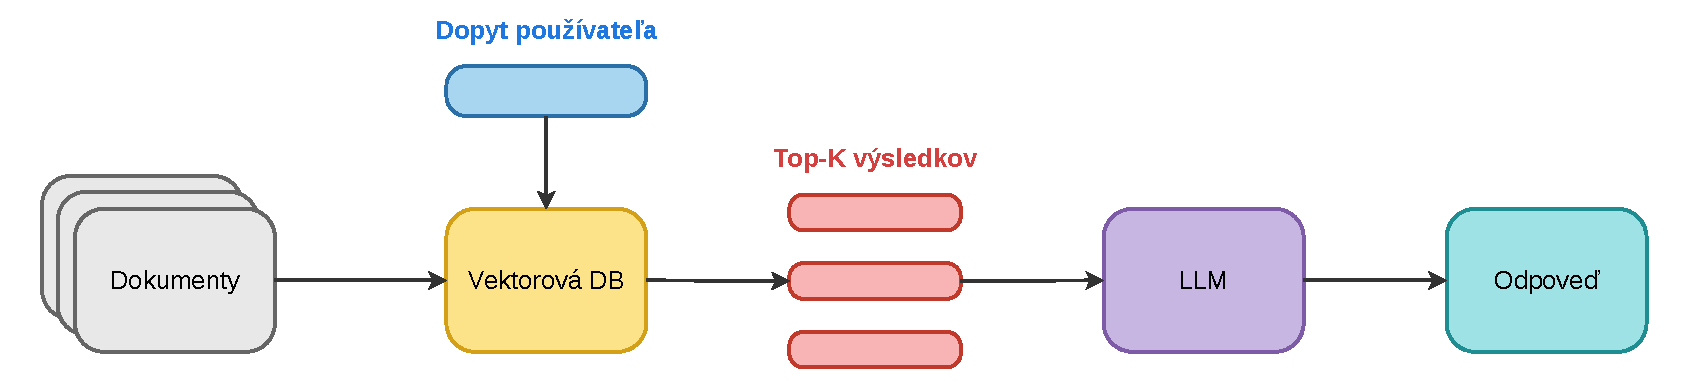
\includegraphics[width=\textwidth]{img/basic_rag_pipeline.pdf}
      \caption{Základný princíp RAG pipeline}
      \label{fig:rag_pipeline}
\end{figure}

Princíp fungovania je taký, že pri každej otázke používateľa, retrieval model
vyhľadá v~znalostnej báze relevantné úseky dokumentov, tie sa vložia do
kontextu \acrshort{llm} spolu s~pôvodnou otázkou a~model na ich základe
vygeneruje odpoveď. Znalostná báza je typicky uložená vo vektorovej databáze,
kde sú dokumenty reprezentované ako číselné vektory (embeddingy) umožňujúce
rýchle vyhľadávanie. Jednou z~populárnych open-source vektorových databáz je
ChromaDB. Ľahká databáza licencovaná pod Apache~2.0, ktorú možno prevádzkovať
lokálne alebo aj v~cloudovom prostredí a~je priamo integrovaná s~frameworkmi
LangChain a~LlamaIndex~\cite{t19}.

Hlavné prínosy \acrshort{rag} oproti čistému \acrshort{llm} sú zníženie
halucinácií dohľadaním odpovedí v~konkrétnych zdrojoch, prístup k~aktuálnym
a~doménovým dátam a teda možnosť odkazovať na zdroj informácie priamo
v~odpovedi.

\subsection{AI asistenti v priemyselnom prostredí}

Priemyselné podniky čelia rastúcemu nedostatku kvalifikovaných pracovníkov
a~potrebe rýchleho zaškolenia nových zamestnancov. Generatívni \acrshort{ai}
asistenti môžu predstavovať súčasť riešenia tohto problému. Fungujú ako
virtuálni mentori priamo na výrobnej linke, kde pracovníkom poskytujú okamžité
odpovede v~prirodzenom jazyku na otázky o~postupoch, riešení porúch alebo
špecifikáciách zariadení~\cite{t20}.

Systém vie prepájať viaceré zdroje dát ako podnikové systémy, tréningové
databázy, prevádzkové dáta a skladať z~nich kontextovo relevantnú odpoveď.
Technická dokumentácia je tak prekladaná do zrozumiteľných pokynov
prispôsobených skúsenostiam konkrétneho pracovníka. Výsledkom je potenciálne
skrátenie času zaškoľovania, zníženie závislosti od rád seniornejších
zamestnancov a~vyššia schopnosť prispôsobiť sa pri zavádzaní nových
technológií.

\section{Typy identifikátorov a ich použitie}

\subsection{QR kódy}
QR kódy sú dvojrozmerné maticové identifikátory optimalizované pre rýchle
čítanie a vysokú hustotu dát. V zmysle použitia v priemysle sa využívajú najmä
na identifikáciu objektov, kde sa vyžaduje uloženie komplexnejších informácií
napr. URL adresy, sériové čísla alebo konfiguračné parametre. Ich výhodou je
silná korekcia chýba, ktorá umožňuje prečítať kód aj pri čiastočnom poškodení
alebo znečistení povrchu.

\subsection{Fiduciálne markery -- AprilTag, ArUco}
Fiduciálne markery sú špeciálne navrhnuté pre potreby počítačového videnia a
robotiky. Na rozdiel od QR kódov nie je ich primárnym cieľom prenos veľkého
objemu dát, ale presná lokalizácia v 3D priestore.

Tieto identifikátory sa vyznačujú predovšetkým vysokou mierou interoperability
s modernými robotickými riešeniami. Vďaka existujúcim knižniciam napr. OpenCV,
ROS je ich integrácia štandardom pri vývoji:
\begin{itemize}
      \item \textbf{Autonómnych robotov:} Kde markery umiestnené v prostredí slúžia ako pevné referenčné body pre rekalibráciu lokalizácie a elimináciu kumulatívnej chyby v mapách.
      \item \textbf{Dronov v skladoch:} Kde umožňujú presné pristávanie na nabíjacích staniciach alebo navigáciu v priestoroch bez signálu GPS, pričom dron dokáže v reálnom čase určiť svoju polohu a náklon voči markeru.
      \item \textbf{Kolaboratívnych robotov:} Pri navádzaní na presnú pozíciu.
\end{itemize}
Identifikátory ako AprilTag a ArUco sú robustné voči zmenám osvetlenia a perspektívnemu skresleniu.

\subsection{3D identifikátory}
V prostrediach priemyselných podnikov a logistických reťazcov, kde môže prísť k
jednoduchému znemožneniu snímania 2D identifikátorov (špinavé, poškodené,
nedostatočné osvetlenie, odrazy svetla), sa ako perspektívne riešenie javia
unikátne 3D identifikátory. Na Fakulte elektrotechniky a informatiky STU bol
vyvinutý systém programaticky generovaných 3D identifikátorov, ktoré sú
optimalizované pre systémy zmiešanej a rozšírenej reality.

\begin{figure}[h]
      \centering
      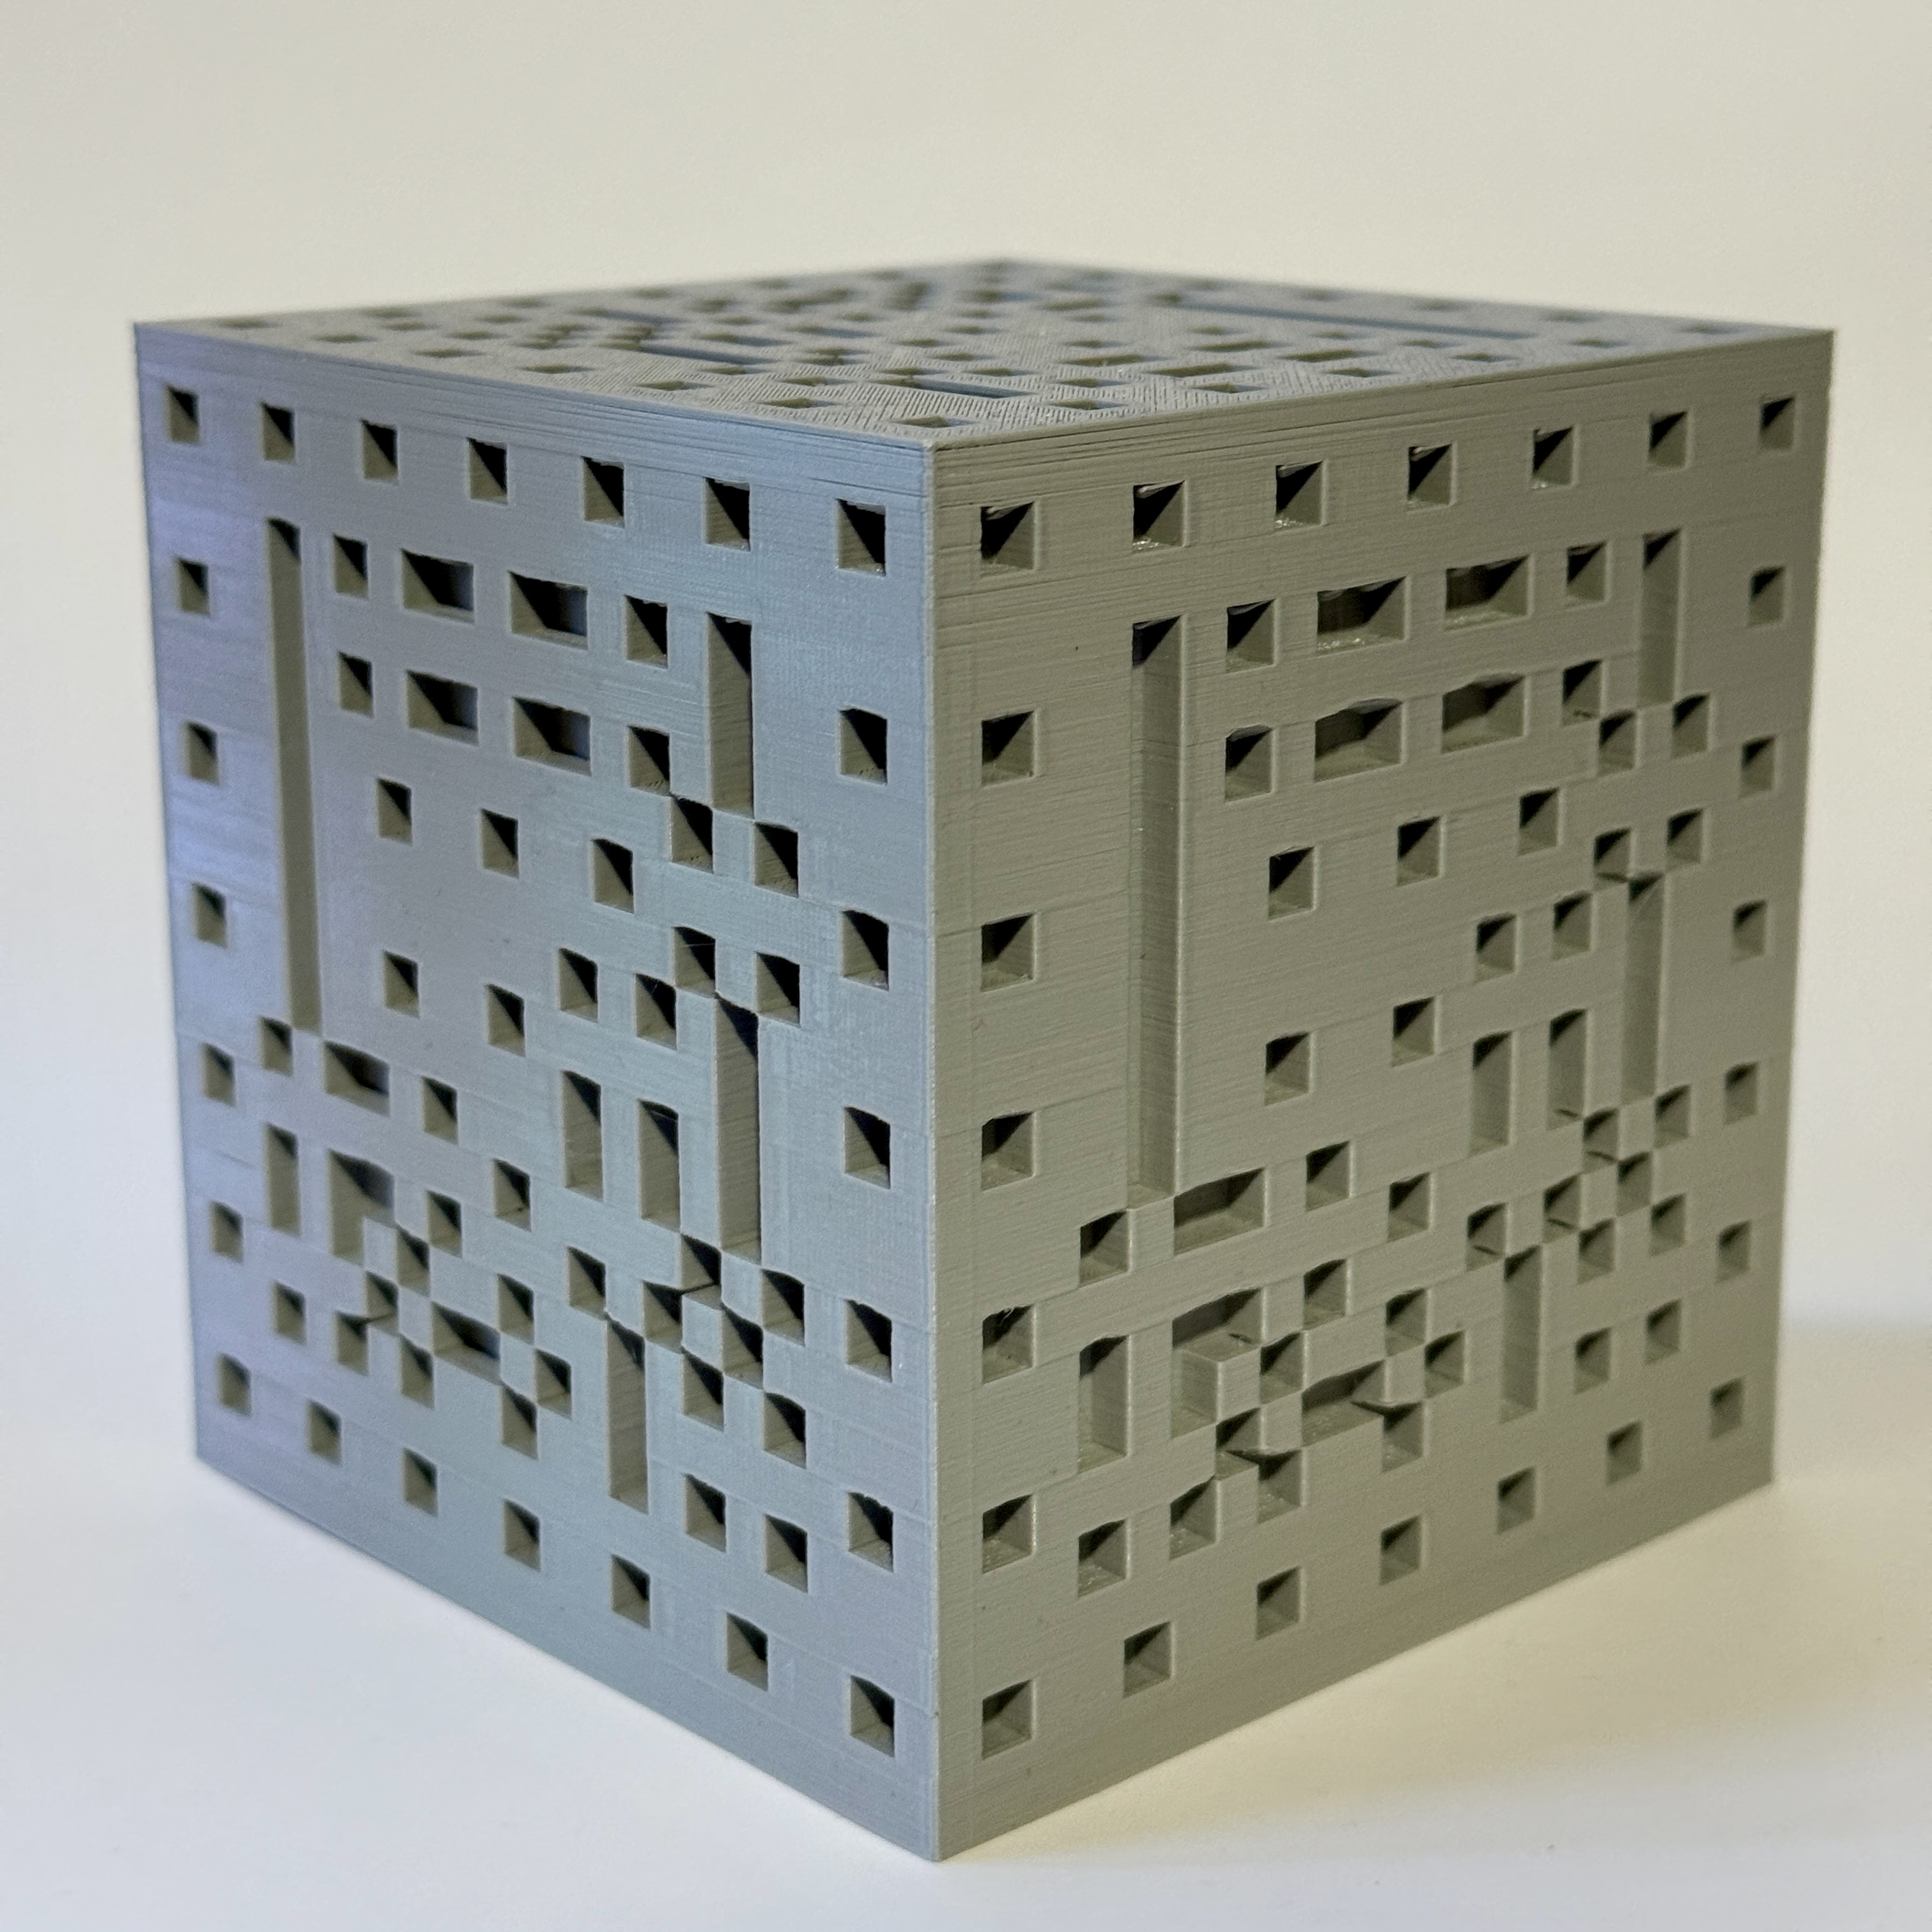
\includegraphics[width=0.45\textwidth]{img/3D_identifikator.jpg}
      \caption{Fyzický 3D identifikátor vyrobený pomocou 3D tlače}
      \label{fig:3d_identifikator}
\end{figure}

\subsubsection{Princíp a štruktúra}
Navrhnutý 3D identifikátor má tvar kocky, ktorá je vnútorne vyskladaná z
menších, unikátnych geometrických elementov. Tieto elementy sú usporiadané v
originálnej štruktúre, ktorá v sebe nesie zakódované informácie.

Hlavné technické výhody tohto riešenia sú:
\begin{itemize}
      \item \textbf{Všesmerová detekcia:} Na rozdiel od 2D QR kódov je možné tieto 3D objekty v systémoch zmiešanej reality spoľahlivo snímať z akéhokoľvek uhla.
      \item \textbf{Odolnosť voči falšovaniu:} Vďaka komplexnej vnútornej členitosti a 3D geometrii sú tieto identifikátory výrazne náročnejšie na replikáciu než bežné 2D identifikátory.
      \item \textbf{Využitie vlastného tvaru:} Sledovanie sa nespolieha len na vizuálny vzor, ale na obrys a priestorovú charakteristiku 3D modelu, čo zvyšuje stabilitu v AR aplikáciách.
\end{itemize}

\section{Špecifikácia požiadaviek systému}

Práca predstavuje moderný prístup k priemyselnému internetu vecí
(\acrshort{iiot}), kde mobilná aplikácia slúži ako primárne rozhranie pre
obsluhu výrobnej linky, prepojené s riadiacim systémom prostredníctvom edge
computing zariadenia umiestneného priamo v prevádzke.

\subsection{Prehľad systému}

V moderných priemyselných prevádzkach narastá tlak na flexibilitu a mobilitu
obsluhy výrobných zariadení. Tradičné riešenia sú spravidla viazané na pevne
umiestnené operátorské panely alebo stolové počítače, čo obmedzuje pohyblivosť
obsluhy a~zvyšuje reakčný čas pri riešení prevádzkových udalostí. Mobilné
zariadenia ponúkajú možnosť prístupu k výrobným systémom odkiaľkoľvek v rámci
areálu závodu. Ich použitie v~kombinácii s~jednoznačnou identifikáciou
zariadení otvára cestu k~bezpečnému a~intuitívnemu ovládaniu výrobnej linky.

Kľúčovou výzvou pri takomto prístupe je spoľahlivé a~jednoznačné spárovanie
mobilného zariadenia s~konkrétnou fyzickou časťou výrobnej linky. Skenovaním
jedinečného identifikátora umiestneného priamo pri zariadení operátor okamžite
nadviaže spojenie a systém presne vie, kto a~ktoré zariadenie ovláda. Toto
spojenie je základom pre bezpečné riadenie, zaznamenávanie operácií a~správu
prístupu viacerých používateľov k rovnakému zariadeniu.

Ďalšou dôležitou oblasťou je správa prístupu pracovníkov s~rôznymi rolami.
Operátor potrebuje priamy prístup k~riadeniu linky, manažér vyžaduje prehľad o dianí vo výrobe, údržbár musí mať garantovaný neprepisovateľný prístup pri servisnom zásahu
a~administrátor spravuje celý systém vrátane schvaľovania registrácie nových používateľov.
Bez jasne definovaného mechanizmu riadenia prístupu by mohlo dôjsť ku konfliktom príkazov
alebo neoprávnenému zásahu do výrobného procesu.

Celá komunikačná vrstva od \acrshort{plc} až po mobilnú aplikáciu prebieha cez
štandardné priemyselné a~webové protokoly. Backendová infraštruktúra je plne
kontajnerizovaná a to umožňuje rýchle nasadenie.
Ovládanie linky je obmedzené výhradne na lokálnu sieť továrne.

Neoddeliteľnou súčasťou systému je inteligentný technický asistent. Asistent
odpovedá na technické otázky obsluhy výhradne na základe dokumentácie
a~manuálov nahratých pre konkrétne zariadenie, čím znižuje závislosť od
papierových príručiek a~skracuje čas potrebný na riešenie prevádzkových
problémov.

\subsection{Popis používateľských rolí}

Systém implementuje riadenie prístupu založené na rolách (\textit{Role-Based
      Access Control}, RBAC). Každý nový používateľ sa musí zaregistrovať a~pred
prvým prihlásením čaká na schválenie administrátorom alebo manažérom, ktorý mu zároveň priradí
príslušnú rolu. Sú definované štyri roly:

\begin{description}
      \item[Operátor:] Základná obsluha výrobnej linky. Prihlasuje sa na konkrétnu linku
            skenovaním ArUco kódu, odosiela riadiace príkazy a~sleduje aktuálny stav zariadenia v~reálnom čase. Nemá prístup
            k~reportom, správe vedomostnej bázy ani správe používateľov. Môže v prípade
            potreby využiť AI asistenta.

      \item[Manažér:] Zameriava sa na sledovanie udalostí. Má prístup
            k~histórii prihlásení jednotlivých operátorov, reportu s logmi a môže spravovať používateľské kontá. Takisto má prístup k~AI asistentovi a môže upravovať vedomostnú bázu.
            Linku priamo neovláda no vidí kto je prihlásený a aké operácie vykonáva.

      \item[Údržbár:] Má exkluzívnu ochranu relácie a žiadny iný používateľ ho nemôže
            odhlásiť z~prihláseného zariadenia, čo zaručuje bezpečnosť počas servisného zásahu.
            Spravuje vedomostnú bázu pre jednotlivé zariadenia, môže upravovať existujúce zariadenia a vytvárať nové.

      \item[Administrátor:] Spravuje celý systém, schvaľuje nové registrácie, priraďuje
            roly, edituje a~odstraňuje používateľské kontá. Má prístup prakticky ku všetkým funkciám systému.
\end{description}

\subsection{Use-case scenáre}

\noindent
\begin{tabularx}{\textwidth}{@{}l X@{}}
      \toprule
      \textbf{ID}    & UC-01: Registrácia a prihlásenie           \\
      \textbf{Aktér} & Všetky roly                                \\
      \textbf{Popis} & Používateľ sa zaregistruje zadaním údajov.
      Kým administrátor neschváli konto, aplikácia zobrazí informáciu o~čakaní na schválenie.
      Po schválení sa používateľ prihlási a~získa prístup.      \\
      \bottomrule
\end{tabularx}

\vspace{6pt}\noindent
\begin{tabularx}{\textwidth}{@{}l X@{}}
      \toprule
      \textbf{ID}    & UC-02: Skenovanie ArUco kódu a spárovanie linky                             \\
      \textbf{Aktér} & Operátor, údržbár, admin                                                           \\
      \textbf{Popis} & Používateľ naskenuje ArUco kód pri zariadení.
      Ak je linka voľná, po potvrdení dialógu sa vytvorí relácia.
      Ak je obsadená, zobrazí sa identita a~rola prihláseného.
      Reláciu neprítomného operátora je možné prevziať, reláciu údržbára prevziať nie je povolené. \\
      \bottomrule
\end{tabularx}

\vspace{6pt}\noindent
\begin{tabularx}{\textwidth}{@{}l X@{}}
      \toprule
      \textbf{ID}    & UC-03: Ovládanie linky                                                                                                                                                                                                  \\
      \textbf{Aktér} & Operátor, údržbár, admin                                                                                                                                                                                                                               \\
      \textbf{Popis} & Aktéri odosielajú príkazy z~ovládacieho panelu.
      Vykonanie príkazu je potvrdené a je zobrazený čas od odoslania po prijatie príkazu zariadením. \\
      \bottomrule
\end{tabularx}

\vspace{6pt}\noindent
\begin{tabularx}{\textwidth}{@{}l X@{}}
      \toprule
      \textbf{ID}    & UC-04: Monitorovanie stavu linky                                                                                        \\
      \textbf{Aktér} & Operátor, údržbár, admin                                                                                                      \\
      \textbf{Popis} & Dashboard zobrazuje procesné dáta z~PLC v~reálnom čase cez WebSocket. Stavy sú farebne kódované podľa normy IEC\,60073. \\
      \bottomrule
\end{tabularx}

\vspace{6pt}\noindent
\begin{tabularx}{\textwidth}{@{}l X@{}}
      \toprule
      \textbf{ID}    & UC-05: Prezeranie logov                                                                                        \\
      \textbf{Aktér} & Manažér, údržbár, admin                                                                                                            \\
      \textbf{Popis} & Je možné prezeranie logov a reportov s filtorvaním podľa časového obdobia a zariadenia. \\
      \bottomrule
\end{tabularx}

\vspace{6pt}\noindent
\begin{tabularx}{\textwidth}{@{}l X@{}}
      \toprule
      \textbf{ID}    & UC-06: Správa vedomostnej bázy                                                                                          \\
      \textbf{Aktér} & Manažér, údržbár, admin                                                                                                          \\
      \textbf{Popis} & Prostredníctvom CRUD operácií sa nahrávajú, upravujú a~odstraňujú dokumenty znalostnej bázy. \\
      \bottomrule
\end{tabularx}

\vspace{6pt}\noindent
\begin{tabularx}{\textwidth}{@{}l X@{}}
      \toprule
      \textbf{ID}    & UC-07: AI asistent                                                                                   \\
      \textbf{Aktér} & Všetky roly                                                                                                        \\
      \textbf{Popis} & Tlačidlom v~rohu každej obrazovky sa spustí chatbot.
      Odpovedá výhradne na základe vedomostnej bázy, či už všeobecnej alebo viazanej ku konkrétnemu zariadeniu. Ak informácia chýba, prizná to. Rozhranie aj odpovede sú lokalizované v~SK a~EN. \\
      \bottomrule
\end{tabularx}

\vspace{6pt}\noindent
\begin{tabularx}{\textwidth}{@{}l X@{}}
      \toprule
      \textbf{ID}    & UC-08: Správa používateľov                                                                                                                \\
      \textbf{Aktér} & Manažér, admin                                                                                                                                     \\
      \textbf{Popis} & Manažér a admin schvaľuje registrácie, priraďuje roly, upravuje a~odstraňuje kontá. Hlavného admina nie je možné odstrániť ani upraviť inou cestou. \\
      \bottomrule
\end{tabularx}

\vspace{6pt}\noindent
\begin{tabularx}{\textwidth}{@{}l X@{}}
      \toprule
      \textbf{ID}    & UC-09: Nastavenia aplikácie                                                                                        \\
      \textbf{Aktér} & Všetky roly                                                                                                        \\
      \textbf{Popis} & V~nastaveniach je možné zmeniť jazyk (SK\,/\,EN) a~vlastné heslo. Zmena jazyka je dostupná aj na prihlasovacej obrazovke. \\
      \bottomrule
\end{tabularx}


\subsection{Funkcionálne požiadavky}

\begin{description}
      \item [FP1:] Aplikácia musí umožniť načítanie unikátneho identifikátora na automatické spárovanie mobilného zariadenia s konkrétnou časťou výrobnej linky.
      \item [FP2:] Používateľ musí mať možnosť odosielať príkazy v riadenom systéme.
      \item [FP3:] Systém musí implementovať verifikáciu kritických príkazov. Po odoslaní požiadavky musí aplikácia čakať na potvrdenie z PLC a vizuálne indikovať úspešné vykonanie zmeny.
      \item [FP4:] Zobrazovanie aktuálnych stavov z PLC.
      \item [FP5:] Implementácia chatbota využívajúceho metódu \textit{Retrieval-Augmented Generation}. Chatbot musí odpovedať na technické otázky výhradne na základe poskytnutej vedomostnej bázy. Ak čerpá z iného zdoja, musí to jasne uviesť.
      \item [FP6:] Plná lokalizácia používateľského rozhrania a odpovedí chatbota v dvoch jazykoch: slovenský (SK) a anglický (EN).
      \item [FP7:] Aplikácia musí implementovať mechanizmus exkluzívnej relácie pre ovládanie konkrétnej výrobnej linky. Po úspešnom prihlásení a spárovaní linky sa vytvorí aktívna relácia viazaná na používateľa. Relácia musí byť udržiavaná periodickým \textit{heartbeat} signálom a automaticky ukončená pri odhlásení.
      \item [FP8:] Pri pokuse o spárovanie linky, ktorá je už obsadená aktívnou reláciou, musí aplikácia používateľovi zobraziť informáciu o existujúcej relácii (používateľa/rola). Nútené ukončenie resp. prevzatie relácie musí byť umožnené v prípade neodhlásenia sa už neprítomnej obsluhy.
      \item [FP9:] Systém musí podporovať prihlásenie používateľov pomocou autentifikácie založenej na JWT. Aplikácia musí implementovať \textit{Role-Based Access Control} (RBAC) s rolami: operátor, manažér, údržbár, admin.
      \item [FP10:] Systém musí ukladať základný log operácií obsahujúci minimálne: čas vykonania, identifikátor používateľa, identifikátor linky, typ akcie/príkazu a výsledok vykonania. Log musí byť dostupný pre roly \textit{manažér}, \textit{údržbár} a \textit{admin}.
\end{description}

\subsection{Nefunkcionálne požiadavky}
Definujú kvalitatívne atribúty, technologické obmedzenia a nároky na
bezpečnosť.

\begin{description}
      \item [NFP1:] Celá backendová infraštruktúra musí byť kontajnerizovaná pomocou nástroja Docker a spustiteľná na edge zariadení.
      \item [NFP2:] Prenos správ v edge infraštruktúre musí prebiehať cez MQTT s QoS 1.
      \item [NFP3:] Latencia príkazov nesmie presiahnuť 250~ms.
      \item [NFP4:] Odpovede AI asistenta musia byť striktne viazané na poskytnutý kontext. Ak informácia v materiáloch chýba, model musí túto skutočnosť priznať.
      \item [NFP5:] Lokálna databáza musí byť konfigurovaná na zachovanie integrity dát aj v prípade náhleho prerušenia napájania edge zariadenia.
      \item [NFP6:] Využitie Docker Compose musí umožňovať rýchle nasadenie identického stacku na iné edge zariadenia napr. v iných závodoch.
      \item [NFP9:] Ovládacie príkazy z môžu prichádzať výhradne z lokálnej siete továrne.
      \item [NFP10:] Backendové služby musia poskytovať štruktúrované logy pre účely diagnostiky.
\end{description}

\subsection{Doménové požiadavky}
Požiadavky plynúce z priemyselného prostredia a použitých technológií.

\begin{description}
      \item [DP1:] Komunikácia s hardvérom PLC musí prebiehať cez natívny protokol S7.
      \item [DP2:] Grafické rozhranie musí dodržiavať priemyselné štandardy pre farebnú indikáciu stavov podľa normy IEC 60073.
      \item [DP3:] Systém si musí zachovať kľúčovú funkcionalitu teda ovládanie linky aj v prípade výpadku pripojenia k internetu.
\end{description}

\section{Voľba technológií}

Výber použitých technológií bol výsledkom posúdenia viacerých faktorov. Medzi
kľúčové kritériá patrili kompatibilita s poskytnutým hardvérom, jednoduchá
integrácia, nízka latencia a schopnosť fungovať v priemyselnom prostredí s
omezenými zdrojmi. V neposlednom rade bola dôležitá aj dostupnosť knižníc a
predchádzajúca skúsenosť s jednotlivými technológiami, čo zásadne urýchli
vývoj.

\subsection{Komunikácia s \acrshort{plc} -- S7 protokol}

Riadiaci systém výrobnej linky je \acrshort{plc} od firmy Siemens, konkrétne
model S7-1200, pre ktorý je natívnym komunikačným protokolom S7. Práve to bolo
primárnym dôvodom jeho výberu. S7 protokol umožňuje priame čítanie a zápis
dátových blokov bez nutnosti zložiej konfigurácie alebo dodatočných licencií.

Alternatívou by bolo aktivovanie servera \acrshort{opcua} priamo v~S7-1200, čo
je síce technicky možné, avšak prináša niekoľko nevýhod. Tými sú vyšší nápor na
výpočtové zdroje \acrshort{plc} s obmedzenou pamäťou, potrebu licencie a
výrazne komplexnejší konfiguračný proces. S7 protokol cez knižnicu
\texttt{node-red-contrib-s7} poskytuje priamy a jednoduchý prístup k~dátam
\acrshort{plc} bez týchto obmedzení.

\begin{itemize}
      \item \textbf{Výhody:} Natívna podpora pre Siemens S7-1200, priamy prístup k~dátovým blokom, nízke vyťažovanie prostriedkov, jednoduchá konfigurácia v~Node-RED.
      \item \textbf{Nevýhody:} Viazanosť na platformu Siemens, absencia štandardizovaného informačného modelu v porovnaní s \acrshort{opcua}.
\end{itemize}

\subsection{Komunikačná middleware vrstva -- Node-RED}

Spojenie medzi \acrshort{plc} a zvyškom systému zabezpečuje Node-RED, nástroj
na programovanie s využitím minima kódu. Bbeží ako Docker kontajner priamo
na edge zariadení v~prevádzke. Node-RED periodicky číta hodnoty
z~\acrshort{plc} prostredníctvom S7 protokolu a publikuje ich do
\acrshort{mqtt} brokera, čím spája svet \acrshort{ot} (\acrshort{plc}, S7) a
\acrshort{it} (\acrshort{mqtt}, backend).

Node-RED bol zvolený z~niekoľkých dôvodov. Disponuje uzlom
\texttt{node-red-contrib-s7} pre priamu komunikáciu so Siemens \acrshort{plc} a
rovnako podporou \acrshort{mqtt}. Toto riešenie je bez potreby písať
rozsiahly kód, čo výrazne skracuje čas konfigurácie. Node-RED tiež dobre zvláda
periodické dotazovanie (polling) \acrshort{plc} a podmienené spúšťanie akcií.

\begin{itemize}
      \item \textbf{Výhody:} Minimum kódu, natívna S7 a \acrshort{mqtt} podpora, jednoduchý deployment v~Dockeri, aktívna komunita s~rozsiahlou knižnicou uzlov.
      \item \textbf{Nevýhody:} Nie je vhodný pre komplexnú biznis logiku, vizuálne toky môžu byť pri väčšom projekte ťažšie udržiavateľné.
\end{itemize}

\subsection{Transportný protokol -- \acrshort{mqtt}}

Pre transport dát medzi edge vrstvou a backendom bol zvolený protokol
\acrshort{mqtt}. Kľúčovým argumentom je jeho nenáročnosť. Protokol bol
navrhnutý pre zariadenia s~obmedzenými zdrojmi a nestabilné siete.

\acrshort{opcua} je komplexný štandard s~bohatým informačným modelom, vstavanou
bezpečnosťou a sémantickým popisom dát. Pre scenár, kde Node-RED číta hodnoty
zo Siemens \acrshort{plc} a odovzdáva ich ďalej na spracovanie, táto komplexnosť
nepredstavuje pridanú hodnotu, ale zbytočnú záťaž. \acrshort{mqtt} broker nasadený v~Dockeri zvládne rovnakú úlohu s~minimálnou náročnosťou na zdroje.

\begin{itemize}
      \item \textbf{Výhody \acrshort{mqtt}:} Nízke nároky na zdroje, jednoduchá architektúra pub/sub, výborná podpora v~Node-RED aj Pythone, \acrshort{qos} úrovne pre spoľahlivosť doručenia.
      \item \textbf{Kedy by bol \acrshort{opcua} lepšou voľbou:} Pri požiadavke na štandardizovaný sémantický popis dát, pri integrácii viacerých zariadení od rôznych výrobcov alebo pri prísnych bezpečnostných požiadavkách.
\end{itemize}

\subsection{Backend -- FastAPI}

Backend aplikácie bol implementovaný v~Pythone s~využitím frameworku FastAPI.
Tvorí \acrshort{api} pre celú mobilnú aplikáciu. Oddelené \acrshort{api}
obsluhuje \acrshort{ai} asistenta vrátane \acrshort{rag} pipeline. Voľba
Pythonu bola prirodzená, pretože knižnice LangChain, ChromaDB a~Ollama sú
súčasťou python ekosystému a ich integrácia je bezproblémová.FastAPI bolo 
zvolené ale aj z~ďaľších praktických dôvodov. Asynchrónna architektúra
(\acrshort{asgi}) umožňuje súbežne obsluhovať požiadavky mobilnej aplikácie aj
dlhotrvajúce volania jazykového modelu bez vzájomného blokovania. Automaticky
generovaná OpenAPI dokumentácia uľahčuje ladenie \acrshort{api} počas vývoja.
Validácia vstupov cez Pydantic redukuje množstvo pomocného kódu. Rolu zohrali
aj predchádzajúce skúsenosti s~týmto frameworkom v bakalarskej práci, čo
výrazne urýchlilo vývoj a umožnilo sa sústrediť na implementáciu biznis logiky
a~integráciu AI asistenta.

\begin{itemize}
      \item \textbf{Výhody:} Asynchrónne spracovanie požiadaviek, automatická OpenAPI dokumentácia, Pydantic validácia, AI knižnice, rýchly vývoj.
      \item \textbf{Nevýhody:} Interpretovaný Python je pomalší oproti kompilovaným jazykom pri \acrshort{cpu}-intenzívnych operáciách.
\end{itemize}

\subsection{Frontend -- Flutter}

Pre mobilnú aplikáciu bol zvolený framework Flutter od spoločnosti Google.
Primárnou cieľovou platformou je Android, avšak Flutter umožňuje z~jednej
kódovej základne generovať aj webovú aplikáciu, desktopovú aplikáciu a iOS aplikáciu, čo otvára možnosť implementácie
administrátorského panelu, či vývoja pre iné platformy bez nutnosti udržiavať samostatný projekt.

Oproti natívnemu vývoju v~Kotline, Flutter ponúka výrazne rýchlejší vývojový
cyklus vďaka funkciám hot reload a hot restart. Vlastný vykresľovací engine
Impeller zaručuje vizuálnu konzistenciu rozhrania naprieč zariadeniami a
operačnými systémami. Bohatá štandardná knižnica widgetov pokrýva väčšinu
potrieb priemyselného ovládacieho rozhrania.

\begin{itemize}
      \item \textbf{Výhody:} Jedna kódová základňa pre Android, iOS aj web, rýchly vývojový cyklus, konzistentné \acrshort{ui}, silná podpora od Google.
      \item \textbf{Nevýhody:} Väčšia veľkosť výslednej aplikácie oproti natívnym riešeniam, pri požiadavke na plnohodnotnú iOS aplikáciu by bolo potrebné doplniť testovanie na Apple zariadeniach.
\end{itemize}

\subsection{Výber identifikátora -- ArUco}

Pre jednoznačnú identifikáciu zariadení bolo v~rámci práce spočiatku
investované značné množstvo času do experimentovania s~3D identifikátormi
navrhnutými študentom FEI. Tieto identifikátory sa spočiatku javili ako vhodné
riešenie, pretože poskytovali vizuálne unikátny vzor, ktorý by teoreticky mohol
byť rozpoznaný pomocou počítačového videnia.

Preto bolo otestovaných niekoľko prístupov k~ich rozpoznávaniu:

\begin{itemize}
      \item \textbf{Template matching a hashing} -- porovnanie snímaného
            povrchu s~uloženými referenčnými vzormi metódami pHash, SSIM
            a~klasický template matching.
      \item \textbf{Extrakcia príznakov ORB s~FLANN matcher} -- rotačne
            invariantné príznaky s~rýchlym vyhľadávaním v~databáze,
            testované na rôznych vzdialenostiach a~uhloch.
      \item \textbf{Analýza mriežky jamiek} -- priama detekcia binárneho
            vzoru v~19$\times$19 mriežke a~porovnanie matíc.
      \item \textbf{Porovnávanie histogramov} -- identifikácia na základe
            distribúcie intenzít.
      \item \textbf{Siamese network} -- ľahká CNN extrahujúca
            128-dimenzionálne príznakové vektory, identifikácia
            na základe cosine similarity.
      \item \textbf{Transfer learning s~MobileNetV3-Small} -- klasifikátor
            exportovaný do TFLite pre nasadenie v~mobilnej aplikácii Flutter,
            trénovaný s~augmentáciou rotácií a~variáciou osvetlenia.
\end{itemize}

Napriek rozsiahlemu experimentovaniu žiadna z~týchto metód neposkytovala
dostatočne spoľahlivé výsledky v~reálnych podmienkach. Systém si vzory vzájomne
zamieňal, pri zmenách osvetlenia alebo pohľadového uhla klesala istota
rozpoznávania pod použiteľnú hranicu, a~príprava každej novej triedy
identifikátora vyžadovala opätovné zbieranie dát a~doladenie modelu.

Z~týchto dôvodov bolo prijaté rozhodnutie použiť štandardizovaný fiduciálny
marker \textbf{ArUco}. Markery ArUco sú binárne štvorcové vzory s~kódovanou
číselnou identitou a~orientáciou, ktoré sú navrhnuté priamo pre spoľahlivú
detekciu počítačovým videním za rôznych svetelných podmienok. Knižnica ArUco je
súčasťou OpenCV a~poskytuje robustné algoritmy detekcie s~korekciou
perspektívy. V~priemyselnom prostredí majú ArUco markery silné zastúpenie,
využívajú ich napríklad automaticky navádzané vozidlá (AGV), upratovacie
autonómne roboty a aj výskumné robotické platformy. Táto rozšírenosť je ďalším
argumentom v~prospech voľby ArUco oproti 3D identifikátorom, ktoré by
vyžadovali vlastný spôsob rozpoznávania. Prípadne by bolo možné
použitie frameworku ako Vuforia, čo by ale značne zvýšilo závislosť
implementácie a údržby a presne tomu sme sa chceli vyhnúť.
%%%% tu pokracovat
\section{Experimentálne porovnanie a výber jazykových modelov}

\subsection{Popis testovaných modelov}

Na účely porovnania bolo vybraných päť lokálne spustiteľných jazykových modelov
dostupných prostredníctvom platformy Ollama. Modely boli zámerne zvolené tak,
aby pokrývali tri veľkostné kategórie: modely do 10 miliárd parametrov, modely
v rozsahu 10 až 15 miliárd parametrov a model s 24 miliardami parametrov.
Cieľom tohto rozloženia bolo analyzovať vzťah medzi veľkosťou modelu, kvalitou
odpovedí a časom odozvy.

\begin{enumerate}

      \item \textbf{llama3.2:3b} \\
            Kompaktný model od spoločnosti Meta s~3 miliardami parametrov zo série Llama~3.2,
            ktorá zahŕňa predtrénované aj inštrukčne doladené generatívne modely vo veľkostiach
            1B a 3B parametrov. Inštrukčne doladené varianty sú optimalizované pre multijazyčné
            konverzačné úlohy vrátane agentického vyhľadávania a sumarizácie.
            Podľa oficiálnej dokumentácie model prekonáva modely Gemma~2 2.6B
            a Phi~3.5-mini v~úlohách ako sledovanie inštrukcií, sumarizácia,
            prepis promptov a používanie nástrojov~\cite{t21}.
            Do testovania bol zaradený ako zástupca najmenšej veľkostnej kategórie
            s~predpokladom najrýchlejšej odozvy.

      \item \textbf{gemma4:e4b} \\
            Model od spoločnosti Google zo série Gemma~4 s~4 miliardami parametrov
            v~kvantizovanej verzii (e4b označuje efektívnu 4-bitovú kvantizáciu).
            Séria Gemma~4 predstavuje najnovšiu generáciu otvorených modelov Google,
            navrhnutú s~dôrazom na multimodálne schopnosti a efektívne nasadenie
            na bežnom spotrebiteľskom hardvéri. Model podporuje dlhé kontextové okno
            a je optimalizovaný pre inštrukčné úlohy vrátane multijazyčných
            konverzačných scenárov~\cite{t22}.
            Do testovania bol zaradený ako zástupca strednej veľkostnej kategórie
            s~priaznivým pomerom výkonu a pamäťovej náročnosti.

      \item \textbf{mistral-nemo:12b} \\
            Model s~12 miliardami parametrov vyvinutý spoločnosťami Mistral AI a NVIDIA.
            Disponuje kontextovým oknom až 128\,000 tokenov a podľa oficiálnej dokumentácie
            dosahuje v~svojej veľkostnej kategórii špičkové výsledky v~oblasti uvažovania,
            znalosti sveta a presnosti generovania kódu. Vďaka štandardnej architektúre je
            plnohodnotnou náhradou modelu Mistral~7B v~existujúcich systémoch~\cite{t23}.
            Do testovania bol zaradený ako zástupca kategórie 10--15 miliárd parametrov.

      \item \textbf{phi4:14b} \\
            Model od spoločnosti Microsoft s~14 miliardami parametrov a kontextovým oknom
            16\,000 tokenov. Je trénovaný na kombinácii syntetických dátových sád,
            filtrovaných verejne dostupných webových zdrojov a akademických kníh
            a dátových sád otázok a odpovedí. Prešiel procesom doladenia pomocou
            supervised fine-tuningu a direct preference optimization s~dôrazom na presné
            sledovanie inštrukcií a bezpečnosť. Podľa oficiálnej dokumentácie je určený
            pre prostredia s~obmedzenými výpočtovými zdrojmi, scenáre s~požiadavkami
            na nízku latenciu a úlohy vyžadujúce uvažovanie a logiku~\cite{t24}.
            Do testovania bol zaradený ako druhý zástupca kategórie 10--15 miliárd parametrov.

      \item \textbf{mistral-small:24b} \\
            Model od spoločnosti Mistral AI s~24 miliardami parametrov a kontextovým oknom
            32\,000 tokenov, ktorý stanovuje nový benchmark v~kategórii modelov do 70B parametrov.
            Podľa oficiálnej dokumentácie dosahuje výkon porovnateľný s~modelmi trojnásobnej
            veľkosti a proprietárnym modelom GPT-4o mini naprieč úlohami v~oblasti kódu,
            matematiky, všeobecných znalostí a sledovania inštrukcií~\cite{t25}.
            Model vyniká multijazyčnou podporou, natívnym volaním funkcií, \acrshort{json} výstupom
            a silnou adherenciou k~systémovým promptom. Vďaka kompaktnej veľkosti je
            nasaditeľný lokálne na bežnom spotrebiteľskom hardvéri a je licencovaný pod Apache~2.0.

\end{enumerate}

\subsection{Metodika testovania}

Testovanie prebiehalo formou automatizovaného benchmarku implementovaného
v~jazyku Python s~využitím knižníc LangChain, ChromaDB a Ollama. Znalostná báza
asistenta vo formáte \texttt{.txt} bola rozdelená na sekcie podľa markerov
\texttt{--- NÁZOV DOKUMENTU: ---} a uložená do vektorovej databázy ChromaDB
s~využitím embedding modelu \texttt{nomic-embed-text}. Pre každú testovú otázku
boli z~vektorovej databázy vytiahnuté tri najrelevantnejšie dokumenty, ktoré
boli spolu s~otázkou odovzdané modelu ako kontext.

Každý model bol otestovaný na sade 14 testovacích otázok rozdelených do troch
kategórií:

\begin{itemize}
      \item \textbf{Faktické otázky} (10 otázok) -- odpoveď je priamo
            obsiahnutá v~znalostnej báze. 6 otázok v~slovenskom
            a 4 otázky v~anglickom jazyku.
      \item \textbf{Otázky vyžadujúce syntézu} (2 otázky) -- správna odpoveď
            vyžaduje kombináciu informácií z~viacerých dokumentov
            znalostnej bázy.
      \item \textbf{Otázky mimo rozsahu} (2 otázky) -- otázky,
            ktorých odpoveď sa v~znalostnej báze nenachádza a
            model by mal odpovedať odmietnutím a odkazom na technika.
\end{itemize}

Na rozdiel od automatických metrík ako ROUGE, ktoré vykazujú nízku spoľahlivosť
pri jazykoch, kde sa využíva skloňovanie, ako je slovenčina, bolo hodnotenie
kvality realizované manuálne. Každá odpoveď bola ohodnotená podľa nasledujúcich
kritérií:

\begin{itemize}
      \item \textbf{Relevancia} (škála 1--5) -- miera, do akej odpoveď
            zodpovedá položenej otázke.
      \item \textbf{Úplnosť} (škála 1--5) -- pokrytie všetkých
            dôležitých bodov správnej odpovede.
      \item \textbf{Zrozumiteľnosť} (škála 1--5) -- zrozumiteľnosť formulácie odpovede.
      \item \textbf{Jazyková správnosť} (škála 1--3) -- či model
            odpovedal v~rovnakom jazyku, v~akom bola položená otázka.
      \item \textbf{Odmietnutie otázky mimo rozsahu} (áno/nie) --
            či model správne odmietol odpovedať na otázku,
            ktorá nie je pokrytá znalostnou bázou.
\end{itemize}

Celkové skóre bolo vypočítané ako vážený priemer jednotlivých kritérií:
relevancia (30\,\%), úplnosť (25\,\%), zrozumiteľnosť (20\,\%) a jazyková
správnosť (25\,\%).

Okrem kvalitatívnych metrík bol pre každú odpoveď zaznamenaný čas odozvy
v~milisekundách. Testovanie prebiehalo na notebookovom hardvéri (\acrshort{cpu}
AMD Ryzen 5 5600H, \acrshort{ram} 32\,GB, \acrshort{gpu} NVIDIA RTX~3060 6\,GB
\acrshort{vram}). Keďže väčšina testovaných modelov presahuje kapacitu
\acrshort{vram}, modely bežali čiastočne alebo úplne na systémovej
\acrshort{ram}, čo predstavuje hardvérovú limitáciu meraní. V~produkčnom
nasadení, na dedikovanom serveri s~dostatočnou \acrshort{vram}, by časy odozvy
boli výrazne nižšie.

\subsection{Výsledky porovnania}

Výsledky hodnotenia všetkých piatich modelov sú zhrnuté
v~tabuľke~\ref{tab:model_comparison}.

\begin{table}[h]
      \centering
      \caption{Výsledky porovnania jazykových modelov}
      \label{tab:model_comparison}
      \renewcommand{\arraystretch}{1.3}
      \begin{tabular}{lccccccc}
            \hline
            \textbf{Model}                         &
            \textbf{\shortstack{Priem.\\čas [ms]}} &
            \textbf{\shortstack{Relev.\\(1--5)}}   &
            \textbf{\shortstack{Úplnosť\\(1--5)}}  &
            \textbf{\shortstack{Zrozum.\\(1--5)}}  &
            \textbf{\shortstack{Jazyk\\(1--3)}}    &
            \textbf{\shortstack{OOS\\odmiet.}}     &
            \textbf{\shortstack{Celk.\\skóre}}                                                                     \\
            \hline
            llama3.2:3b                            & 4\,536  & 2,29 & 2,21 & 2,50 & 2,14 & 100\,\% & 2,63          \\
            gemma4:e4b                             & 11\,165 & 4,86 & 4,86 & 5,00 & 3,00 & 100\,\% & \textbf{4,92} \\
            mistral-nemo:12b                       & 15\,217 & 4,07 & 4,07 & 4,29 & 2,86 & 100\,\% & 4,29          \\
            phi4:14b                               & 20\,039 & 2,00 & 2,00 & 2,07 & 2,79 & 100\,\% & 2,68          \\
            mistral-small:24b                      & 35\,801 & 1,86 & 1,86 & 1,86 & 3,00 & 100\,\% & 2,65          \\
            \hline
      \end{tabular}
\end{table}

\begin{table}[h]
      \centering
      \caption{Priemerná relevancia podľa typu otázky a jazyka}
      \label{tab:model_detail}
      \renewcommand{\arraystretch}{1.3}
      \begin{tabular}{lcccccc}
            \hline
            \textbf{Model}                         &
            \textbf{\shortstack{Faktická\\otázka}} &
            \textbf{Syntéza}                       &
            \textbf{\shortstack{Mimo\\rozsahu}}    &
            \textbf{SK}                            &
            \textbf{EN}                                                               \\
            \hline
            llama3.2:3b                            & 1,70 & 2,50 & 5,00 & 2,12 & 2,50 \\
            gemma4:e4b                             & 5,00 & 4,00 & 5,00 & 4,88 & 4,83 \\
            mistral-nemo:12b                       & 4,20 & 2,50 & 5,00 & 4,62 & 3,33 \\
            phi4:14b                               & 1,40 & 2,00 & 5,00 & 2,00 & 2,00 \\
            mistral-small:24b                      & 1,40 & 1,00 & 5,00 & 2,00 & 1,67 \\
            \hline
      \end{tabular}
\end{table}

% ------------------------------------------------------------

\subsection{Analýza výsledkov a výber modelu}

Z~výsledkov testovania vyplýva, že model \textbf{gemma4:e4b} dosiahol najvyššie
celkové skóre 4,92/5,0 spomedzi všetkých testovaných modelov. Model vykazoval
konzistentne vysokú kvalitu odpovedí naprieč všetkými typmi otázok aj oboma
testovacími jazykmi, pričom jeho priemerný čas odozvy 11\,165\,ms bol
v~podmienkach notebookového hardvéru prijateľný a takmer trojnásobne nižší
v~porovnaní s~modelom mistral-small:24b.

Prekvapivým zistením je, že modely phi4:14b a mistral-small:24b opakovane
odmietali odpovedať na otázky, ktorých odpovede boli v~znalostnej báze
jednoznačne obsiahnuté. Tento jav naznačuje, že \acrshort{rag} pipeline nepodal
týmto modelom dostatočne relevantný kontext, čo mohlo byť spôsobené odlišnou
citlivosťou modelov na formát vstupného kontextu.

Všetky testované modely dosiahli 100\,\% úspešnosť pri odmietaní otázok mimo
rozsahu znalostnej bázy, čo potvrdzuje správne fungovanie systémového promptu
z~hľadiska bezpečnosti systému.

\subsubsection{Overenie na cloudovom hardvéri}

V~nadväznosti na merania realizované lokálne bolo vybrané testovanie vykonaných
aj na platforme RunPod.io, ktorá poskytuje prístup k~výkonným GPU serverom
formou platby za využitý čas. Cieľom bolo overiť, do akej miery hardvérová
limitácia skresľuje závery o~reálnej použiteľnosti modelov v~produkcii.

Výsledky potvrdili predpoklad, na dedikovanom serverovom hardvéri s~dostatočnou
\acrshort{vram} klesol priemerný čas odozvy na menej ako 8 sekúnd, čo je pre
interaktívne použitie výrazne prijateľnejšia hodnota. Kvalita odpovedí pritom
zostala nezmenená, čo je v~súlade s~očakávaním. Model generuje rovnaký výstup
nezávisle od hardvéru, rozdiel sa prejaví iba v~latencii.

\subsubsection{Záverečné rozhodnutie o architektúre AI asistenta}

Napriek tomu, že výsledky testovania lokálnych modelov boli z~kvalitatívneho
hľadiska uspokojivé, cloudové overenie odhalilo zásadné ekonomické obmedzenie
tohto prístupu. Modely, ktoré dosahujú dostatočnú kvalitu odpovedí, si pre
produkčné nasadenie vyžadujú dedikovaný GPU server s~dostatočnou
\acrshort{vram}. Prevádzkové náklady takéhoto riešenia nie sú pre projekt tohto
rozsahu rentabilné.

V prípade väčších organizácií s~vyšším objemom požiadaviek by mohlo byť
zmysluplné investovať do vlastného serverového hardvéru. Stále však bude
výhodnosť vlastného servera s GPU závislá od konkrétneho objemu požiadaviek.
Pre nízky až stredný objem požiadaviek, je určite ekonomicky výhodnejšie
využívať cloudové \acrshort{api} s~modelom per-token, kde náklady sú
priamoúmerné skutočnému využitiu a nevyžadujú si vysokú počiatočnú investíciu.

Z~týchto dôvodov bolo rozhodnuté opustiť prístup lokálnych \acrshort{llm} a
prejsť na volanie externého \acrshort{api}. Na výber je niekoľko poskytovateľov
ako OpenAI, Google, Anthropic a iní veľkí hráči v oblasti AI. My sme zvolili
\acrshort{api} od spoločnosti Anthropic, nakoľko v poslednej dobe zaznamenali
výraznejší pokrok v porovnaní s konkurenciou. Tento prístup zabezpečuje prístup
k~výkonným jazykovým modelom bez nutnosti prevádzkovať vlastný server, pričom
náklady sa platia priamoúmerne skutočnému využitiu. \acrshort{rag} pipeline a
znalostná báza zostávajú zachované v~pôvodnej podobe. Kontextové dokumenty sú
naďalej vyhľadávané lokálne z~vektorovej databázy a odovzdávané modelu ako
súčasť promptu. Mení sa iba vrstva generovania odpovede, ktorá prechádza
z~lokálne bežiaceho modelu na cloudové \acrshort{api}.

\section{Návrh architektúry systému}
Systém je navrhnutý ako distribuovaná aplikácia skladajúca sa z viacerých
vzájomne prepojených vrstiev. Každá vrstva plní špecifickú úlohu a komunikuje
so susednými vrstvami prostredníctvom jasne definovaných rozhraní. Jadro
systému beží na edge zariadení umiestenom priamo v prevádzke a zabezpečuje plnú
funkčnosť aj bez pripojenia k internetu. Mobilná aplikácia komunikuje výhradne
v rámci lokálnej siete závodu a v súčasnosti sa pripojenie na internet využíva
len pre účely AI asistenta. Ak by sme využívali lokálne spustiteľný jazykový
model, komunikácia s AI asistentom by prebiehala výhradne v rámci lokálnej
siete a celý systém by bol izolovaný. Nasledujúce podkapitoly popisujú celkovú
štruktúru systému, spôsob nasadenia jednotlivých komponentov, ich vzájomnú
komunikáciu a formát ukladania dát.

\subsection{Architektúra komponentov systému}
Systém sa skladá z piatich hlavných komponentov. Prvým je mobilná aplikácia
Flutter, ktorá slúži ako primárne rozhranie pre obsluhu. Druhým je backendová
vrstva tvorená dvoma službami FastAPI. Hlavnou službou zabezpečujúcou
autentifikáciu, správu relácií, riadenie zariadení a samostatnou službou AI
asistenta s RAG pipeline. Tretím komponentom je MQTT broker Mosquitto, ktorý
sprostredkúva asynchrónnu komunikáciu medzi backendom a Node-RED. Štvrtým je
Node-RED, ktorý premosťuje svet priemyselnej komunikácie so svetom IT a
periodicky číta dáta z PLC prostredníctvom S7 protokolu. Posledným komponentom
je samotné PLC Siemens S7-1200, ktoré fyzicky ovláda zariadenia na výrobnej
linke. Všetky tieto komponenty okrem mobilnej aplikácie bežia ako Docker
kontajnery na edge zariadení. Jediné externé volanie smeruje z AI služby na
rozhranie Anthropic API.

\begin{figure}[h]
      \centering
      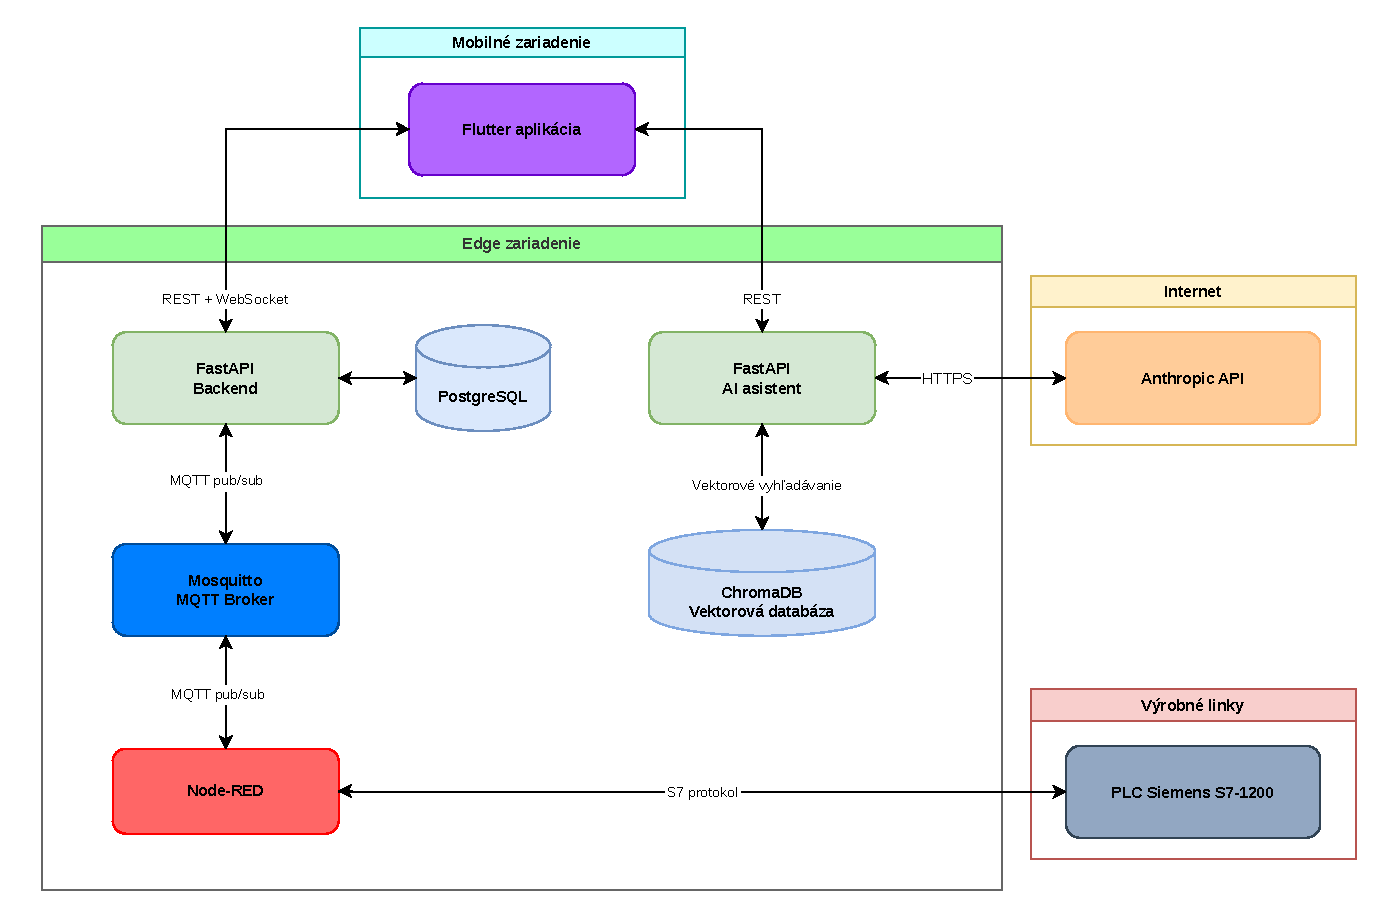
\includegraphics[width=\textwidth]{img/architektura_systemu.pdf}
      \caption{Diagram architektúry systému a komunikácia medzi komponentmi}
      \label{fig:architecture}
\end{figure}

Mobilná aplikácia komunikuje s hlavnou FastAPI službou cez REST API a prijíma
aktualizácie stavu zariadení cez WebSocket. Príkazy odoslané z aplikácie putujú
cez backend do MQTT brokera a ďalej do Node-RED, ktorý ich zapíše do PLC.
Spätná väzba prechádza tou istou cestou v opačnom smere. Dáta zo senzorov PLC
číta Node-RED periodicky a publikuje ich do príslušných MQTT tém, odkiaľ ich
backend preposiela pripojeným klientom cez WebSocket.

\subsection{Fyzická topológia systému}
Fyzická topológia systému vychádza z požiadavky na lokálnu prevádzku bez
závislosti od externej infraštruktúry. Celá komunikácia prebieha v rámci
lokálnej siete medzi mobilnými zariadeniami, edge zariadením a riadiacimi
systémami výrobných liniek. Schéma fyzickej architektúry je znázornená na
obrázku \ref{fig:fyzicka_architektura}.

\begin{figure}[H]
      \centering
      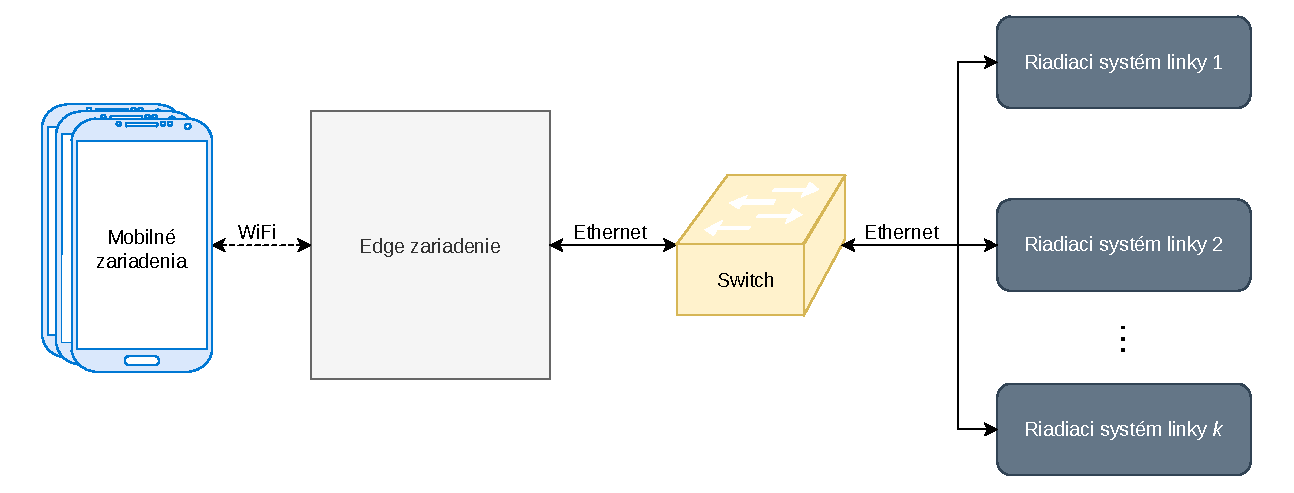
\includegraphics[width=\textwidth]{img/fyzicka_architektura.pdf}
      \caption{Fyzická topológia systému}
      \label{fig:fyzicka_architektura}
\end{figure}

Mobilné zariadenia sa pripájajú k edge zariadeniu bezdrôtovo cez WiFi. Voľba
bezdrôtového pripojenia vychádza z charakteru práce operátora, ktorý sa
pohybuje po výrobnej hale a potrebuje mať prístup k systému kdekoľvek v jej
dosahu. Edge zariadenie je prepojené s Ethernet switchom, na ktorý sú napojené
riadiace systémy výrobných liniek. Edge zariadenie plní úlohu centrálneho uzla,
beží na ňom backend aj AI asistent a všetka logika spracovania príkazov sa
vykonáva lokálne (okrem LLM, v práci sme zvolili externé API). Architektúra
počíta s pripojením viacerých riadiacich systémov, čo umožňuje rozšírenie na
ďalšie výrobné linky bez zmeny základnej topológie. V súčasnej implementácii je
na switch napojený jeden riadiaci systém Siemens S7-1200.

\subsection{Štruktúra MQTT tém}

Komunikácia medzi backend službou, Node-RED a zariadeniami prebieha cez
štruktúrované MQTT témy. Všetky témy zdieľajú spoločný prefix \texttt{plc}, za
ktorým nasleduje identifikátor zariadenia vo formáte \texttt{device\_\{id\}},
kde \texttt{id} zodpovedá ArUco identifikátoru fyzického zariadenia. Táto
štruktúra umožňuje systému jednoznačne smerovať správy na konkrétne zariadenie
a zároveň odberateľom filtrovať témy.

\dirtree{%
      .1 plc/.
      .2 device\_\{id\}/.
      .3 data \DTcomment{stav zariadenia \quad Node-RED -> backend}.
      .3 status \DTcomment{online/offline \quad\quad Node-RED -> backend}.
      .3 commands/.
      .4 \{prikaz\} \DTcomment{riadiaci prikaz \quad backend -> Node-RED}.
}

\begin{table}[H]
      \centering
      \caption{Prehľad MQTT tém}
      \label{tab:mqtt_topics}
      \begin{tabular}{|l|l|l|p{5cm}|}
            \hline
            \textbf{Téma} & \textbf{Vydavateľ} & \textbf{Odberateľ} & \textbf{Popis}                              \\
            \hline
            \texttt{plc/device\_\{id\}/data}
                          & Node-RED           & Backend            & Aktuálne hodnoty premenných zariadenia      \\
            \hline
            \texttt{plc/device\_\{id\}/status}
                          & Node-RED           & Backend            & Stav pripojenia zariadenia (online/offline) \\
            \hline
            \texttt{plc/device\_\{id\}/commands/\#}
                          & Backend            & Node-RED           & Riadiaci príkaz smerovaný na zariadenie     \\
            \hline
      \end{tabular}
\end{table}

Backend pri štarte subscribuje na tému \texttt{plc/\#}, čím prijíma správy zo
všetkých zariadení naraz. Node-RED subscribuje selektívne len na témy
\texttt{commands} pre zariadenia, ktoré spravuje. Príkazy sú publikované s QoS
1, čím je zaručené doručenie aspoň raz.

\section{Implementácia backendu}
Backend systému tvorí dvojica nezávislých FastAPI služieb bežiacich v prostredí
Docker. Hlavná služba zabezpečuje autentifikáciu, správu zariadení a
spracovanie príkazov. Druhá služba je určená výhradne pre AI asistenta. Obe
služby komunikujú s mobilnou aplikáciou cez REST API, pričom hlavná služba
poskytuje navyše WebSocket kanál pre aktualizácie stavu zariadení. V
nasledujúcich podkapitolách popisujeme implementáciu jednotlivých funkcionalít
backendu, začínajúc autentifikáciou a RBAC, cez API endpointy, mechanizmus
relácií, životný cyklus príkazov a ochranu prístupu až po generátor ArUco
identifikátorov a export identifikátorov vo formáte STL vhodnom pre 3D tlač.

\subsection{Autentifikácia a RBAC}

Systém používa autentifikáciu pomocou JWT tokenov podľa štandardu OAuth2. Po
úspešnom prihlásení server vygeneruje token podpísaný zdieľaným tajným kľúčom
algoritmom HS256. Token obsahuje identifikátor používateľa a čas vypršania
platnosti. Heslá sú uložené výhradne ako bcrypt hash.

Registrácia je verejne dostupná, avšak nový účet je predvolene neaktívny.
Prístup do systému získa až po schválení administrátorom, ktorý zároveň priradí
rolu. Táto dvojfázová registrácia zabraňuje neoprávnenému vstupu do systému.

Oprávnenia sú riadené štyrmi rolami. Každý chránený endpoint deklaruje
požadovanú rolu ako FastAPI závislosť, čo umožňuje jednotnú kontrolu prístupu
bez duplicitnej logiky.

\begin{lstlisting}[language=Python, caption={Závislosti pre kontrolu rolí}]
async def get_line_operator(user: User = Depends(get_current_user)):
    _ensure_role(user, {"operator", "admin", "maintenance"})
    return user

async def get_manager_or_admin(user: User = Depends(get_current_user)):
    _ensure_role(user, {"manager", "admin"})
    return user
\end{lstlisting}

\begin{tabular}{|l|c|c|c|c|}
      \hline
      \textbf{Funkcia}                   & \textbf{Operátor} & \textbf{Manažér} & \textbf{Údržbár} & \textbf{Admin} \\
      \hline
      Dashboard, nastavenia, AI asistent & \checkmark        & \checkmark       & \checkmark       & \checkmark     \\
      \hline
      ArUco skenovanie a ovládanie linky & \checkmark        &                  & \checkmark       & \checkmark     \\
      \hline
      Zoznam a správa zariadení          &                   & \checkmark       & \checkmark       & \checkmark     \\
      \hline
      Log príkazov                       &                   & \checkmark       & \checkmark       & \checkmark     \\
      \hline
      Znalostná báza                     &                   & \checkmark       & \checkmark       & \checkmark     \\
      \hline
      Správa používateľov                &                   & \checkmark       &                  & \checkmark     \\
      \hline
\end{tabular}

\subsection{API endpointy}
Backend poskytuje REST API rozdelené do šiestich skupín podľa funkčnej oblasti.
Endpointy pre AI asistenta sú dostupné na samostatnej službe počúvajúcej na
porte 8100, ostatné na porte 8000. Okrem REST komunikácie poskytuje backend
WebSocket endpoint pre real-time aktualizácie stavu zariadenia.

\begin{table}[H]
      \centering
      \caption{Prehľad API endpointov}
      \label{tab:api_endpoints}
      \resizebox{\textwidth}{!}{%
            \begin{tabular}{|l|l|l|l|}
                  \hline
                  \textbf{Metóda} & \textbf{Endpoint}                   & \textbf{Popis}                  & \textbf{Rola}            \\
                  \hline
                  \multicolumn{4}{|l|}{\textit{Autentifikácia — /auth}}                                                              \\
                  \hline
                  POST            & /auth/login                         & Prihlásenie, vracia JWT token   & —                        \\
                  POST            & /auth/register                      & Registrácia nového účtu         & —                        \\
                  GET             & /auth/me                            & Aktuálny prihlásený používateľ  & všetci                   \\
                  PUT             & /auth/me                            & Úprava mena a priezviska        & všetci                   \\
                  POST            & /auth/change-password               & Zmena hesla                     & všetci                   \\
                  \hline
                  \multicolumn{4}{|l|}{\textit{Zariadenia — /plc}}                                                                   \\
                  \hline
                  GET             & /plc/devices                        & Zoznam zariadení                & všetci                   \\
                  POST            & /plc/devices                        & Vytvorenie zariadenia           & admin, údržbár           \\
                  GET             & /plc/devices/\{id\}                 & Detail zariadenia               & všetci                   \\
                  PUT             & /plc/devices/\{id\}                 & Úprava zariadenia               & admin, údržbár           \\
                  DELETE          & /plc/devices/\{id\}                 & Vymazanie zariadenia            & admin, údržbár           \\
                  POST            & /plc/devices/\{id\}/command/\{cmd\} & Odoslanie príkazu               & admin, údržbár, operátor \\
                  GET             & /plc/stats                          & Dashboard štatistiky            & všetci                   \\
                  WS              & /plc/ws/\{id\}                      & Real-time stav + príkazy        & všetci                   \\
                  \hline
                  \multicolumn{4}{|l|}{\textit{Relácie — /device-sessions}}                                                          \\
                  \hline
                  POST            & /device-sessions/\{id\}/join        & Prihlásenie na zariadenie       & admin, údržbár, operátor \\
                  POST            & /device-sessions/\{id\}/leave       & Odhlásenie zo zariadenia        & všetci                   \\
                  \hline
                  \multicolumn{4}{|l|}{\textit{Logy — /command-logs}}                                                                \\
                  \hline
                  GET             & /command-logs                       & Logy s filtrami                 & admin, manažér, údržbár  \\
                  GET             & /command-logs/device/\{id\}         & Logy zariadenia                 & admin, manažér, údržbár  \\
                  \hline
                  \multicolumn{4}{|l|}{\textit{Používatelia — /users}}                                                               \\
                  \hline
                  GET             & /users                              & Zoznam používateľov             & admin, manažér           \\
                  POST            & /users/\{id\}/approve               & Schválenie + rola               & admin, manažér           \\
                  PUT             & /users/\{id\}                       & Úprava účtu                     & admin, manažér           \\
                  POST            & /users/\{id\}/reset-password        & Reset hesla                     & admin, manažér           \\
                  DELETE          & /users/\{id\}                       & Vymazanie účtu                  & admin, manažér           \\
                  \hline
                  \multicolumn{4}{|l|}{\textit{ArUco — /aruco}}                                                                      \\
                  \hline
                  GET             & /aruco/next-id                      & Nasledujúce voľné ID            & všetci                   \\
                  GET             & /aruco/preview/\{id\}               & Náhľad markera                  & všetci                   \\
                  GET             & /aruco/png/\{id\}                   & Stiahnutie markera ako PNG      & všetci                   \\
                  GET             & /aruco/stl/\{id\}                   & Stiahnutie markera ako STL      & všetci                   \\
                  \hline
                  \multicolumn{4}{|l|}{\textit{AI asistent — port 8100}}                                                             \\
                  \hline
                  POST            & /chat                               & Správa AI asistentovi           & všetci                   \\
                  GET             & /kb                                 & Zoznam záznamov znalostnej bázy & admin, manažér, údržbár  \\
                  POST            & /kb                                 & Pridanie záznamu                & admin, manažér, údržbár  \\
                  POST            & /kb/upload                          & Nahranie súboru do KB           & admin, manažér, údržbár  \\
                  DELETE          & /kb/\{id\}                          & Vymazanie záznamu               & admin, manažér, údržbár  \\
                  \hline
            \end{tabular}%
      }
\end{table}

\subsection{Mechanizmus relácií}
Pred ovládaním zariadenia sa musí používateľ na neho prihlásiť. Relácia je
väzba medzi používateľom a zariadením, ktorá zabraňuje súčasnému ovládaniu
jedného zariadenia viacerými používateľmi. Na každom zariadení môže byť aktívna
práve jedna relácia.

Prihlásenie prebieha volaním \texttt{POST /devices/\{id\}/login}. Backend
overí, či je zariadenie voľné. Ak áno, vytvorí novú reláciu. Ak je zariadenie
obsadené, správanie závisí od parametra \texttt{force} a od roly aktuálneho
držiteľa relácie. Zariadenie obsadené používateľom s rolou údržbára nemôže byť
prebraté žiadnym iným používateľom. Táto ochrana zabraňuje prerušeniu
servisného zásahu operátorom. Vlastnú reláciu môže ukončiť prihlásený
používateľ odhlásením sa. Cudziu reláciu môže ukončiť výhradne administrátor.

\subsection{Životný cyklus príkazu}

Príkaz prechádza niekoľkými vrstvami systému, kým sa prejaví na fyzickom
zariadení. Používateľ ho môže odoslať dvoma cestami: cez REST endpoint alebo
cez WebSocket spojenie.

Pri WebSocket ceste backend príkaz najskôr overí voči konfigurácii zariadenia.
Kontroluje sa existencia príkazu a pre numerické a výčtové typy aj platnosť
hodnoty. Ak zariadenie nemá konfiguráciu definovanú, validácia sa preskočí.
REST endpoint validáciu nevykonáva a príkaz odošle priamo.

Po validácii backend publikuje správu na MQTT tému
\texttt{plc/device\_\{id\}/commands/\{cmd\}}. Mosquitto broker správu doručí
Node-RED, ktorý ju preloží do S7 protokolu a zapíše príslušnú premennú v PLC.
Volajúci dostane späť potvrdenie \texttt{command\_ack} s príznakom úspechu
doručenia na broker. Toto potvrdenie nezaručuje vykonanie príkazu na PLC.
Skutočná zmena stavu sa prejaví v ďalšom cykle čítania, keď Node-RED publikuje
aktualizované hodnoty na tému \texttt{plc/device\_\{id\}/data} a backend ich
pošle cez WebSocket do aplikácie.

Každý príkaz je bez ohľadu na výsledok zaznamenávaný do tabuľky
\texttt{command\_logs} s identifikátorom používateľa, zariadenia, zdrojovým
kanálom a príznakom úspechu doručenia.

\subsection{Ochrana prístupu k zariadeniu}

V priemyselnom prostredí je bezpečnosť kritická požiadavka. Aktivácia
zariadenia počas servisného zásahu môže spôsobiť poranenie alebo poškodenie.
Systém preto implementuje mechanizmus exkluzívneho prístupu, ktorý zabraňuje
súčasnému ovládaniu zariadenia viacerými používateľmi.

Na každom zariadení môže byť aktívna práve jedna relácia. Pokus o prihlásenie
na obsadené zariadenie skončí chybou \texttt{409 occupied}, pričom odpoveď
obsahuje informáciu o tom, kto zariadenie práve používa. Tým má nový používateľ
možnosť kontaktovať aktuálneho držiteľa pred prípadným prevzatím.

Osobitné postavenie má rola údržbára. Reláciu údržbára nemôže ukončiť ani
prevziať žiadny iný používateľ bez ohľadu na parameter \texttt{force}. Táto
ochrana vychádza z bezpečnostných požiadaviek priemyselného prostredia — ak
údržbár pracuje pri zariadení, nikto iný nesmie zariadenie uviesť do chodu.

\begin{lstlisting}[language=Python, caption={Ochrana relácie údržbára}]
if active.user.role == "maintenance":
    raise HTTPException(409, "maintenance_locked")
\end{lstlisting}

Pre ostatné roly systém umožňuje núdzové prevzatie zariadenia parametrom
\texttt{force=true}. Táto možnosť je určená pre prípad, keď sa predošlý
používateľ zabudol odhlásiť. Aktuálna relácia sa ukončí a vytvorí sa nová.
Každé prevzatie je zaznamenané v logoch príkazov, čo umožňuje spätné dohľadanie
zodpovednosti.

\subsection{Generátor ArUco markerov a export do STL}

Pre výrobu fyzických markerov bola implementovaná vlastná Python trieda
\texttt{ArucoSTLGeneratorVoxelOptimized}, ktorá generuje STL súbor určený na
dvojfarebnú 3D tlač. Model je navrhnutý tak, aby farebné priradenie v sliceri
bolo čo najjednoduchšie.

\begin{figure}[h]
      \centering
      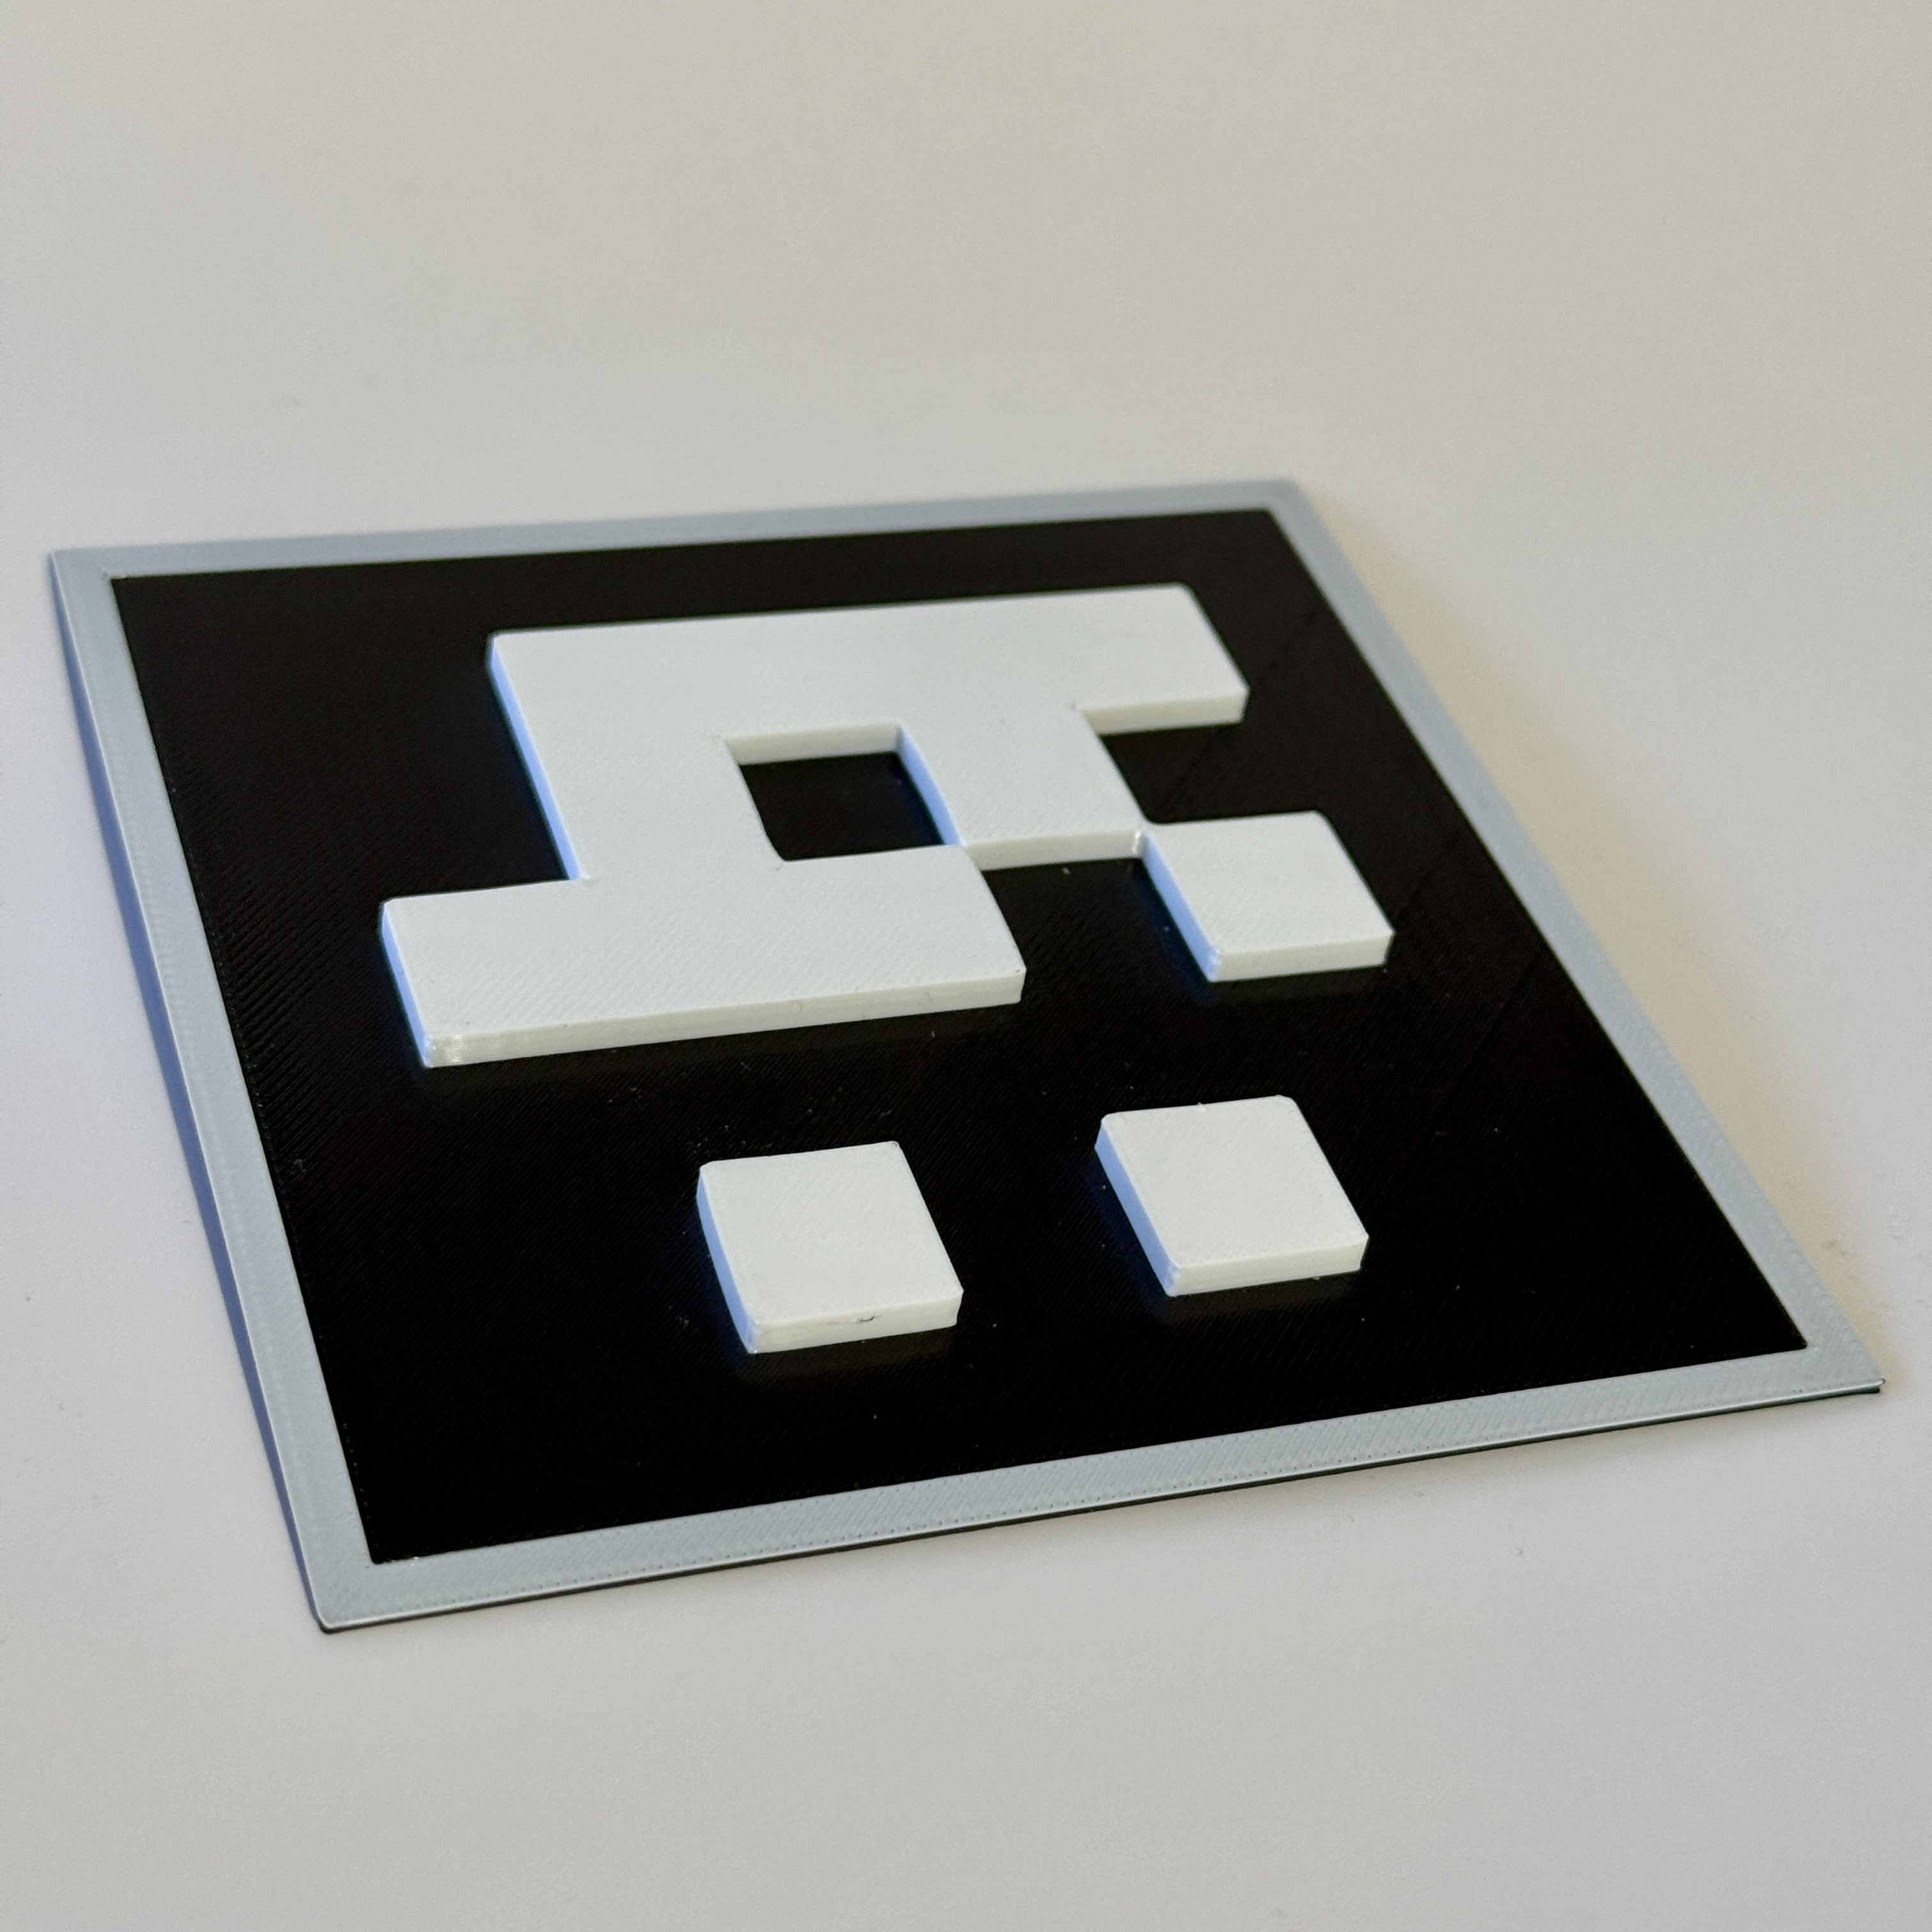
\includegraphics[width=0.45\textwidth]{img/ArUco3D.jpg}
      \caption{ArUco marker tlačený z vygenerovaného STL modelu}
      \label{fig:Aruco3D}
\end{figure}

Povrch modelu je rozdelený do troch výškových úrovní. Čierne bunky markera sú
na základnej výške \texttt{base\_height\_mm}, ohraničovací rám je o
\texttt{border\_height\_offset\_mm} vyšší a biele bunky sú vyvýšené o
\texttt{white\_height\_mm}. Pri predvolených hodnotách dosahujú čierne bunky
výšku 1\,mm a biele 3\,mm.

\section{Implementácia AI asistenta}

Asistent je implementovaný ako samostatná FastAPI služba bežiaca na porte 8100
v rámci vlastného Docker stacku. Disponuje vlastnou PostgreSQL databázou pre
záznamy znalostnej bázy a ChromaDB pre vektorové úložisko. Jediné externé
sieťové volanie celej aplikácie smeruje na Anthropic API pre volanie jazykového
modelu.

\subsection{RAG pipeline}

Spracovanie každej správy prebieha v niekoľkých krokoch. Najprv sa vykonajú dva
vyhľadávacie dotazy do ChromaDB: zariadenie-špecifický s filtrom podľa
\texttt{device\_aruco\_id} a všeobecný bez filtra, pričom každý vráti najviac
tri najbližšie záznamy. Následne prebehne voliteľné vyhľadávanie na webe
pomocou DuckDuckGo. Zo získaných kontextov, metadát relácie a histórie
konverzácie sa zostaví systémový prompt, ktorý sa odošle na Claude API spolu s
poslednou správou používateľa.

\subsection{Embedovací model}

Na generovanie vektorových reprezentácií textov sa používa model
\texttt{nomic-embed-text} spúšťaný lokálne cez Ollama. Model beží v rámci
Docker stacku na edge zariadení a nevyžaduje pripojenie na internet. ChromaDB
využíva kosínusovú podobnosť ako metriku vyhľadávania. Každý záznam znalostnej
bázy sa indexuje ako reťazec \texttt{title + content} pri vytvorení aj
aktualizácii.

\subsection{Systémový prompt}

Asistent vystupuje pod menom PLEXO. Systémový prompt existuje v slovenskej aj
anglickej verzii podľa jazyka relácie a pred každým volaním modelu sa naplní
nasledujúcimi sekciami:

\begin{itemize}
      \item \textbf{AKTUÁLNA RELÁCIA} — meno a rola prihláseného používateľa, prípadne zariadenie na ktoré je prihlásený.
      \item \textbf{KONTEXT PRE ZARIADENIE} — výsledky vyhľadávania z ChromaDB filtrované podľa ArUco ID zariadenia.
      \item \textbf{VŠEOBECNÝ KONTEXT} — výsledky vyhľadávania bez filtra zariadenia.
      \item \textbf{VÝSLEDKY Z INTERNETU} — výstupy z DuckDuckGo, ak boli nájdené.
\end{itemize}

Pravidlá v prompte zakazujú vymýšľanie faktov a nariaďujú asistentovi, aby sa
pri prvej správe stručne predstavil. V ďalších správach konverzácie sa
predstavenie preskakuje.

\subsection{Správa konverzácie}

Server je bezstavový. História konverzácie sa neukladá na strane servera, ale
je súčasťou každého požiadavku zo strany klienta. Služba prijíma pole správ vo
formáte \texttt{\{role, content\}} a pri zostavovaní volania zahŕňa posledných
desať výmen. Tento prístup nevyžaduje žiadne serverové úložisko relácií a
zjednodušuje škálovanie.

\subsection{Správa znalostnej bázy}

Znalostná báza je tvorená textovými záznami uloženými v PostgreSQL. Každý
záznam má názov, obsah a voliteľne priradené ArUco ID zariadenia. Toto
priradenie umožňuje vyhľadávanie obsahu filtrovaného pre konkrétne zariadenie,
čo zvyšuje presnosť odpovedí pri otázkach viazaných na konkrétny stroj.

Pri každom vytvorení alebo úprave záznamu sa jeho vektorová reprezentácia
synchronizuje do ChromaDB operáciou \texttt{upsert}. Mazanie záznamu zrkadlovo
odstráni aj príslušný vektor. Okrem manuálneho zadania textu API podporuje
nahranie súboru vo formáte \texttt{.txt}, čo umožňuje import existujúcej
technickej dokumentácie.

\section{Implementácia frontendu}

Frontend je implementovaný vo Flutter s podporou platformy Android ako
primárneho cieľa a webového prehliadača pre administrátorský panel. Zdieľa
takmer všetok kód medzi platformami s výnimkou ArUco skenovania, kde sú použité
platformovo špecifické implementácie.

\subsection{Stavový manažment}

Aplikácia používa knižnicu Riverpod so vzorcom \texttt{StateNotifier}.
Centrálnym poskytovateľom je \texttt{authProvider}, ktorý uchováva JWT token,
objekt prihláseného používateľa a príznaky stavu autentifikácie. Pri štarte
aplikácie sa volá \texttt{tryRestoreSession}, ktorá overí uložený token volaním
\texttt{/auth/me}. Ak je token platný, relácia sa obnoví. Pri chybe siete sa
použijú záložné údaje z lokálneho úložiska, čo umožňuje obmedzený offline
prístup.

Chatový asistent má vlastného poskytovateľa \texttt{chatProvider}, ktorý
udržiava zoznam správ a informáciu o práve aktívnom zariadení. Táto informácia
sa nastavuje pri otvorení stránky ovládania zariadenia a vymazáva pri odchode.

\subsection{ArUco skenovanie}

Skenovanie prebieha v natívnom kóde prostredníctvom balíčka
\texttt{opencv\_dart}. Každý snímok z kamery dorazí vo formáte YUV420, z
ktorého sa extrahuje kanál Y ako grayscale obraz. Samotná detekcia beží v Dart
izolovanom vlákne pomocou \texttt{Isolate.run}, čím sa zabráni blokovaniu
vykresľovacieho vlákna.

V izolante sa vytvorí detektor s predefinovaným slovníkom
\texttt{DICT\_5X5\_250} a zavolá sa \texttt{detectMarkers}. Pre každý
detekovaný marker sa vypočíta plocha Shoelaceovým vzorcom a stred ako relatívna
poloha v obraze. Výstupom je zoznam detegovaných markerov zoradených od
najväčšieho po najmenší, kde väčšia plocha znamená bližší marker. Príznak
\texttt{\_isProcessing} zabraňuje spusteniu ďalšej detekcie kým prebieha
predchádzajúca.

\subsection{WebSocket pripojenie}

Po načítaní zariadenia sa nadväzuje WebSocket spojenie cez balíček
\texttt{web\_socket\_channel}. Server posiela tri typy správ: heartbeat, ktorý
sa ignoruje, potvrdenie príkazu \texttt{command\_ack} a aktualizáciu hodnôt
premenných. Pri chybe alebo zatvorení spojenia sa po dvoch sekundách
automaticky pokúsi o znovupripojenie.

Odosielanie príkazu funguje tak, že sa na WebSocket pošle JSON správa
\texttt{\{command, value\}} a spustí sa päťsekundový časovač. Ak sa do tohto
času zmení sledovaná premenná na zariadení, používateľovi sa zobrazí snackbar s
potvrdenou hodnotou a nameranou latenciou. Ak časovač vyprší skôr, zobrazí sa
chybové hlásenie.

\subsection{Používateľské rozhranie podľa roly}

Viditeľnosť prvkov rozhrania je riadená pomocnými metódami triedy
\texttt{AuthUser}. Každá metóda vracia booleovskú hodnotu na základe role
prihláseného používateľa. Prehľad priradenia je uvedený v
tabuľke~\ref{tab:rbac}.

V bočnom paneli webového rozhrania sa položky navigácie filtrujú dynamicky.
Napríklad položka správy zariadení sa zobrazí iba ak platí
\texttt{canViewDevices}, tlačidlo konfigurácie zariadenia na stránke ovládania
sa zobrazí iba ak platí \texttt{canManageDevices}. Týmto spôsobom sa rovnaká
logika RBAC z backendu premietne aj do rozhrania bez potreby duplikovania
podmienok na viacerých miestach.

\section{Aplikácia a jej funkcionality}

\subsection{Skener ArUco identifikátorov}
\textbf{Dostupné pre:} operátor, technik, manažér, administrátor

Skener ArUco identifikátorov slúži ako primárny spôsob prihlásenia sa na
konkrétne zariadenie. Používateľ namieri kameru mobilného zariadenia na ArUco
identifikátor umiestnený priamo na fyzickom zariadení a systém ho automaticky
identifikuje. Po úspešnom naskenovaní je používateľ priradený k danému
zariadeniu a získava prístup k jeho monitorovaniu a ovládaniu. Tento prístup
eliminuje manuálne vyhľadávanie zariadení a zabezpečuje, že používateľ pracuje
s tým správnym zariadením.

\subsection{Generátor ArUco identifikátorov}
\textbf{Dostupné pre:} technik, manažér, administrátor

Pri zakladaní nového zariadenia v systéme aplikácia automaticky vygeneruje
unikátny ArUco identifikátor, ktorý jednoznačne identifikuje dané zariadenie.
Identifikátor je možné exportovať vo formáte PNG pre bežnú tlač alebo vo
formáte STL ako trojrozmerný model vhodný na 3D tlač, pričom biela časť kódu je
vystúpená a čierna zapustená. Fyzická značka sa následne umiestni na
zariadenie, čím sa prepojí záznam v systéme s reálnym zariadením v prevádzke.

\subsection{Monitoring a ovládanie zariadení}
\textbf{Dostupné pre:} operátor, technik, administrátor

Monitoring a ovládanie zariadení predstavuje hlavnú funkcionalitu aplikácie. Po
prihlásení na zariadenie má používateľ k dispozícii prehľad aktuálneho stavu
zariadenia v reálnom čase. Môže sledovať stavy senzorov, aktuálny režim
prevádzky, stav v ktorom sa zariadenie nachádza, a iné. Okrem sledovania stavu
môže používateľ zariadenie aj priamo ovládať, napríklad spustiť alebo zastaviť
cyklus, zmeniť smer pohybu či vykonať reset. Všetky zmeny sa prejavia rádovo v
desiatkach milisekúnd, čo umožňuje rýchlu reakciu na aktuálnu situáciu v
prevádzke. Systém zároveň zaznamenáva históriu vykonaných príkazov pre potreby
kontroly a auditu.

\subsection{Virtuálny asistent PLEXO}
\textbf{Dostupné pre:} operátor, technik, manažér, administrátor

Virtuálny asistent PLEXO je inteligentný pomocník dostupný priamo v aplikácii.
Používatelia môžu klásť otázky prirodzeným jazykom, napríklad o aktuálnom stave
zariadenia, postupe pri riešení poruchy alebo pokynoch na údržbu. Asistent
odpovedá na základe znalostnej bázy vytvorenej pre konkrétne zariadenia a
prevádzku. Vďaka tomu má operátor alebo technik potrebné informácie vždy po
ruke, bez nutnosti listovať v technickej dokumentácii. Asistent komunikuje v
jazyku nastavenom používateľom v nastaveniach aplikácie.

\subsection{Správa používateľov}
\textbf{Dostupné pre:} manažér, administrátor

Správa používateľov poskytuje oprávneným osobám nástroje na riadenie prístupu
do systému. Manažér alebo administrátor môže vytvárať nové používateľské účty,
upravovať existujúce, prideľovať príslušné roly podľa pracovného zaradenia a v
prípade potreby účty odstrániť resp. deaktivovať. Systém rolí zabezpečuje, že
každý používateľ vidí a môže vykonávať iba tie akcie, ktoré zodpovedajú jeho
pracovnej pozícii, čím sa minimalizuje riziko neoprávneného zásahu do
prevádzky.

\subsection{Správa zariadení}
\textbf{Dostupné pre:} technik, manažér, administrátor

Správa zariadení umožňuje udržiavať databázu zariadení aktuálnu a v súlade so
skutočným stavom prevádzky. Oprávnený používateľ môže do systému pridať nové
zariadenie, nastaviť jeho parametre a vygenerovať preň ArUco identifikátor.
Existujúce zariadenia je možné upravovať, resp. meniť, čo sa zobrazuje v
ovládacom paneli zariadenia. Taktiež je možné ich zo systému odstrániť, ak boli
vyradené z prevádzky. Vďaka tejto funkcionalite systém vždy odráža reálny stav
zariadení v podniku.

\subsection{Správa znalostnej bázy}
\textbf{Dostupné pre:} technik, manažér, administrátor

Znalostnú bázu tvorí súbor informácií, z ktorých čerpá virtuálny asistent PLEXO
pri odpovedaní na otázky používateľov. Oprávnení používatelia môžu obsah
znalostnej bázy priebežne pridávať nové dokumenty, upravovať existujúce záznamy
alebo odstraňovať zastarané informácie. Kvalita a aktuálnosť znalostnej bázy
priamo ovplyvňuje relevantnosť a presnosť odpovedí asistenta, preto je jej
pravidelná údržba dôležitou súčasťou prevádzky systému.

\subsection{Nastavenia}
\textbf{Dostupné pre:} operátor, technik, manažér, administrátor

Každý používateľ má možnosť prispôsobiť si aplikáciu podľa vlastných
preferencií. V nastaveniach môže zmeniť jazyk rozhrania, ktorý sa automaticky
uplatní aj na komunikáciu s virtuálnym asistentom PLEXO. Zároveň má možnosť
zmeniť si svoje prístupové heslo. Tieto nastavenia sú viazané na konkrétny
používateľský účet a zostávajú zachované aj po opätovnom prihlásení.

\section{Testovanie a meranie}

\subsection{Overenie splnenia špecifikácie}

\subsection{Latencia vykonania príkazov}

\subsection{ArUco detekcia}

\subsection{Kvalita odpovedí asistenta}

